% Options for packages loaded elsewhere
\PassOptionsToPackage{unicode}{hyperref}
\PassOptionsToPackage{hyphens}{url}
%
\documentclass[
]{article}
\usepackage{amsmath,amssymb}
\usepackage{iftex}
\ifPDFTeX
  \usepackage[T1]{fontenc}
  \usepackage[utf8]{inputenc}
  \usepackage{textcomp} % provide euro and other symbols
\else % if luatex or xetex
  \usepackage{unicode-math} % this also loads fontspec
  \defaultfontfeatures{Scale=MatchLowercase}
  \defaultfontfeatures[\rmfamily]{Ligatures=TeX,Scale=1}
\fi
\usepackage{lmodern}
\ifPDFTeX\else
  % xetex/luatex font selection
\fi
% Use upquote if available, for straight quotes in verbatim environments
\IfFileExists{upquote.sty}{\usepackage{upquote}}{}
\IfFileExists{microtype.sty}{% use microtype if available
  \usepackage[]{microtype}
  \UseMicrotypeSet[protrusion]{basicmath} % disable protrusion for tt fonts
}{}
\makeatletter
\@ifundefined{KOMAClassName}{% if non-KOMA class
  \IfFileExists{parskip.sty}{%
    \usepackage{parskip}
  }{% else
    \setlength{\parindent}{0pt}
    \setlength{\parskip}{6pt plus 2pt minus 1pt}}
}{% if KOMA class
  \KOMAoptions{parskip=half}}
\makeatother
\usepackage{xcolor}
\usepackage[margin=1in]{geometry}
\usepackage{color}
\usepackage{fancyvrb}
\newcommand{\VerbBar}{|}
\newcommand{\VERB}{\Verb[commandchars=\\\{\}]}
\DefineVerbatimEnvironment{Highlighting}{Verbatim}{commandchars=\\\{\}}
% Add ',fontsize=\small' for more characters per line
\usepackage{framed}
\definecolor{shadecolor}{RGB}{248,248,248}
\newenvironment{Shaded}{\begin{snugshade}}{\end{snugshade}}
\newcommand{\AlertTok}[1]{\textcolor[rgb]{0.94,0.16,0.16}{#1}}
\newcommand{\AnnotationTok}[1]{\textcolor[rgb]{0.56,0.35,0.01}{\textbf{\textit{#1}}}}
\newcommand{\AttributeTok}[1]{\textcolor[rgb]{0.13,0.29,0.53}{#1}}
\newcommand{\BaseNTok}[1]{\textcolor[rgb]{0.00,0.00,0.81}{#1}}
\newcommand{\BuiltInTok}[1]{#1}
\newcommand{\CharTok}[1]{\textcolor[rgb]{0.31,0.60,0.02}{#1}}
\newcommand{\CommentTok}[1]{\textcolor[rgb]{0.56,0.35,0.01}{\textit{#1}}}
\newcommand{\CommentVarTok}[1]{\textcolor[rgb]{0.56,0.35,0.01}{\textbf{\textit{#1}}}}
\newcommand{\ConstantTok}[1]{\textcolor[rgb]{0.56,0.35,0.01}{#1}}
\newcommand{\ControlFlowTok}[1]{\textcolor[rgb]{0.13,0.29,0.53}{\textbf{#1}}}
\newcommand{\DataTypeTok}[1]{\textcolor[rgb]{0.13,0.29,0.53}{#1}}
\newcommand{\DecValTok}[1]{\textcolor[rgb]{0.00,0.00,0.81}{#1}}
\newcommand{\DocumentationTok}[1]{\textcolor[rgb]{0.56,0.35,0.01}{\textbf{\textit{#1}}}}
\newcommand{\ErrorTok}[1]{\textcolor[rgb]{0.64,0.00,0.00}{\textbf{#1}}}
\newcommand{\ExtensionTok}[1]{#1}
\newcommand{\FloatTok}[1]{\textcolor[rgb]{0.00,0.00,0.81}{#1}}
\newcommand{\FunctionTok}[1]{\textcolor[rgb]{0.13,0.29,0.53}{\textbf{#1}}}
\newcommand{\ImportTok}[1]{#1}
\newcommand{\InformationTok}[1]{\textcolor[rgb]{0.56,0.35,0.01}{\textbf{\textit{#1}}}}
\newcommand{\KeywordTok}[1]{\textcolor[rgb]{0.13,0.29,0.53}{\textbf{#1}}}
\newcommand{\NormalTok}[1]{#1}
\newcommand{\OperatorTok}[1]{\textcolor[rgb]{0.81,0.36,0.00}{\textbf{#1}}}
\newcommand{\OtherTok}[1]{\textcolor[rgb]{0.56,0.35,0.01}{#1}}
\newcommand{\PreprocessorTok}[1]{\textcolor[rgb]{0.56,0.35,0.01}{\textit{#1}}}
\newcommand{\RegionMarkerTok}[1]{#1}
\newcommand{\SpecialCharTok}[1]{\textcolor[rgb]{0.81,0.36,0.00}{\textbf{#1}}}
\newcommand{\SpecialStringTok}[1]{\textcolor[rgb]{0.31,0.60,0.02}{#1}}
\newcommand{\StringTok}[1]{\textcolor[rgb]{0.31,0.60,0.02}{#1}}
\newcommand{\VariableTok}[1]{\textcolor[rgb]{0.00,0.00,0.00}{#1}}
\newcommand{\VerbatimStringTok}[1]{\textcolor[rgb]{0.31,0.60,0.02}{#1}}
\newcommand{\WarningTok}[1]{\textcolor[rgb]{0.56,0.35,0.01}{\textbf{\textit{#1}}}}
\usepackage{longtable,booktabs,array}
\usepackage{calc} % for calculating minipage widths
% Correct order of tables after \paragraph or \subparagraph
\usepackage{etoolbox}
\makeatletter
\patchcmd\longtable{\par}{\if@noskipsec\mbox{}\fi\par}{}{}
\makeatother
% Allow footnotes in longtable head/foot
\IfFileExists{footnotehyper.sty}{\usepackage{footnotehyper}}{\usepackage{footnote}}
\makesavenoteenv{longtable}
\usepackage{graphicx}
\makeatletter
\def\maxwidth{\ifdim\Gin@nat@width>\linewidth\linewidth\else\Gin@nat@width\fi}
\def\maxheight{\ifdim\Gin@nat@height>\textheight\textheight\else\Gin@nat@height\fi}
\makeatother
% Scale images if necessary, so that they will not overflow the page
% margins by default, and it is still possible to overwrite the defaults
% using explicit options in \includegraphics[width, height, ...]{}
\setkeys{Gin}{width=\maxwidth,height=\maxheight,keepaspectratio}
% Set default figure placement to htbp
\makeatletter
\def\fps@figure{htbp}
\makeatother
\setlength{\emergencystretch}{3em} % prevent overfull lines
\providecommand{\tightlist}{%
  \setlength{\itemsep}{0pt}\setlength{\parskip}{0pt}}
\setcounter{secnumdepth}{-\maxdimen} % remove section numbering
\newlength{\cslhangindent}
\setlength{\cslhangindent}{1.5em}
\newlength{\csllabelwidth}
\setlength{\csllabelwidth}{3em}
\newlength{\cslentryspacingunit} % times entry-spacing
\setlength{\cslentryspacingunit}{\parskip}
\newenvironment{CSLReferences}[2] % #1 hanging-ident, #2 entry spacing
 {% don't indent paragraphs
  \setlength{\parindent}{0pt}
  % turn on hanging indent if param 1 is 1
  \ifodd #1
  \let\oldpar\par
  \def\par{\hangindent=\cslhangindent\oldpar}
  \fi
  % set entry spacing
  \setlength{\parskip}{#2\cslentryspacingunit}
 }%
 {}
\usepackage{calc}
\newcommand{\CSLBlock}[1]{#1\hfill\break}
\newcommand{\CSLLeftMargin}[1]{\parbox[t]{\csllabelwidth}{#1}}
\newcommand{\CSLRightInline}[1]{\parbox[t]{\linewidth - \csllabelwidth}{#1}\break}
\newcommand{\CSLIndent}[1]{\hspace{\cslhangindent}#1}
\ifLuaTeX
  \usepackage{selnolig}  % disable illegal ligatures
\fi
\IfFileExists{bookmark.sty}{\usepackage{bookmark}}{\usepackage{hyperref}}
\IfFileExists{xurl.sty}{\usepackage{xurl}}{} % add URL line breaks if available
\urlstyle{same}
\hypersetup{
  pdftitle={Additional tools},
  pdfauthor={Giovanni Saraceno},
  hidelinks,
  pdfcreator={LaTeX via pandoc}}

\title{Additional tools}
\author{Giovanni Saraceno}
\date{}

\begin{document}
\maketitle

{
\setcounter{tocdepth}{2}
\tableofcontents
}
\begin{Shaded}
\begin{Highlighting}[]
\FunctionTok{library}\NormalTok{(tidyverse)}
\FunctionTok{library}\NormalTok{(dplyr)}
\FunctionTok{library}\NormalTok{(ggplot2)}
\end{Highlighting}
\end{Shaded}

\hypertarget{assumptions-in-hypothesis-testing}{%
\subsection{Assumptions in hypothesis
testing}\label{assumptions-in-hypothesis-testing}}

The methods for computing the confidence intervals and hypothesis
testing via the t-test are correct assuming that the variable under
study follows a normal distribution. However, in practice it can happen
that the frequency distribution does not follow a normal distribution or
that the variances of groups are not equal. Hence, it is fundamental in
practice to check that data satisfy this assumption. In general, we can
list the following possible approaches.

\begin{itemize}
\tightlist
\item
  If the sample size is sufficiently large and the violations of
  hypothesis are not extreme, the statistical procedures could be still
  applied and give reasonable results. Note that this is not suggesting
  to blindly ignore the violations of assumptions.
\item
  Transformations of variables: applying some function to the data can
  satisfy the assumptions (logaritmic, arcsin, square root, inverse,
  \ldots).
\item
  \emph{Non-parameteric} methods: these methods do not require model
  assumptions, such as the normality assumtion.
\end{itemize}

\hypertarget{normality-assumption}{%
\subsubsection{Normality assumption}\label{normality-assumption}}

Consider the \texttt{penguin} data set

\begin{Shaded}
\begin{Highlighting}[]
\FunctionTok{library}\NormalTok{(palmerpenguins)}
\FunctionTok{data}\NormalTok{(penguins)}
\FunctionTok{str}\NormalTok{(penguins)}
\end{Highlighting}
\end{Shaded}

\begin{verbatim}
## tibble [344 x 8] (S3: tbl_df/tbl/data.frame)
##  $ species          : Factor w/ 3 levels "Adelie","Chinstrap",..: 1 1 1 1 1 1 1 1 1 1 ...
##  $ island           : Factor w/ 3 levels "Biscoe","Dream",..: 3 3 3 3 3 3 3 3 3 3 ...
##  $ bill_length_mm   : num [1:344] 39.1 39.5 40.3 NA 36.7 39.3 38.9 39.2 34.1 42 ...
##  $ bill_depth_mm    : num [1:344] 18.7 17.4 18 NA 19.3 20.6 17.8 19.6 18.1 20.2 ...
##  $ flipper_length_mm: int [1:344] 181 186 195 NA 193 190 181 195 193 190 ...
##  $ body_mass_g      : int [1:344] 3750 3800 3250 NA 3450 3650 3625 4675 3475 4250 ...
##  $ sex              : Factor w/ 2 levels "female","male": 2 1 1 NA 1 2 1 2 NA NA ...
##  $ year             : int [1:344] 2007 2007 2007 2007 2007 2007 2007 2007 2007 2007 ...
\end{verbatim}

Consider that we want to compare the bill length of penguins from the
species ``Adelie'' and ``Gentoo'', assuming that they have equal
variance.

\begin{Shaded}
\begin{Highlighting}[]
\NormalTok{id\_a }\OtherTok{\textless{}{-}} \FunctionTok{which}\NormalTok{(penguins}\SpecialCharTok{$}\NormalTok{species}\SpecialCharTok{==}\StringTok{"Adelie"} \SpecialCharTok{\&} \SpecialCharTok{!}\FunctionTok{is.na}\NormalTok{(penguins}\SpecialCharTok{$}\NormalTok{bill\_length\_mm))}
\NormalTok{mu\_a }\OtherTok{\textless{}{-}} \FunctionTok{mean}\NormalTok{(penguins}\SpecialCharTok{$}\NormalTok{bill\_length\_mm[id\_a], }\AttributeTok{na.rm =} \ConstantTok{TRUE}\NormalTok{)}
\NormalTok{sd\_a }\OtherTok{\textless{}{-}} \FunctionTok{sd}\NormalTok{(penguins}\SpecialCharTok{$}\NormalTok{bill\_length\_mm[id\_a], }\AttributeTok{na.rm =} \ConstantTok{TRUE}\NormalTok{)}
\NormalTok{id\_g }\OtherTok{\textless{}{-}} \FunctionTok{which}\NormalTok{(penguins}\SpecialCharTok{$}\NormalTok{species}\SpecialCharTok{==}\StringTok{"Gentoo"}\SpecialCharTok{\&} \SpecialCharTok{!}\FunctionTok{is.na}\NormalTok{(penguins}\SpecialCharTok{$}\NormalTok{bill\_length\_mm))}
\NormalTok{mu\_g }\OtherTok{\textless{}{-}} \FunctionTok{mean}\NormalTok{(penguins}\SpecialCharTok{$}\NormalTok{bill\_length\_mm[id\_g], }\AttributeTok{na.rm =} \ConstantTok{TRUE}\NormalTok{)}
\NormalTok{sd\_g }\OtherTok{\textless{}{-}} \FunctionTok{sd}\NormalTok{(penguins}\SpecialCharTok{$}\NormalTok{bill\_length\_mm[id\_g], }\AttributeTok{na.rm =} \ConstantTok{TRUE}\NormalTok{)}
\FunctionTok{print}\NormalTok{(}\FunctionTok{paste0}\NormalTok{(}\StringTok{"Adelie: "}\NormalTok{,mu\_a, }\StringTok{" ("}\NormalTok{, sd\_a, }\StringTok{")"}\NormalTok{))}
\end{Highlighting}
\end{Shaded}

\begin{verbatim}
## [1] "Adelie: 38.7913907284768 (2.66340484836862)"
\end{verbatim}

\begin{Shaded}
\begin{Highlighting}[]
\FunctionTok{print}\NormalTok{(}\FunctionTok{paste0}\NormalTok{(}\StringTok{"Chinstrap: "}\NormalTok{, mu\_g, }\StringTok{" ("}\NormalTok{, sd\_g, }\StringTok{")"}\NormalTok{))}
\end{Highlighting}
\end{Shaded}

\begin{verbatim}
## [1] "Chinstrap: 47.5048780487805 (3.08185737211429)"
\end{verbatim}

In this case, it is appropriate to perform a t.test considering as null
hypothesis \(H_0: \mu_A = \mu_C\) versus \(H_0: \mu_A \not= \mu_C\).
This test assumes that the two populations are normally distributed.

\begin{Shaded}
\begin{Highlighting}[]
\NormalTok{adelie }\OtherTok{\textless{}{-}}\NormalTok{ penguins}\SpecialCharTok{$}\NormalTok{bill\_length\_mm[id\_a]}
\NormalTok{gentoo }\OtherTok{\textless{}{-}}\NormalTok{ penguins}\SpecialCharTok{$}\NormalTok{bill\_length\_mm[id\_g]}
\end{Highlighting}
\end{Shaded}

In order to evaluate the normality assumption we can investigate the
distribution of data using graphical tools, such as boxplots and
histograms, to verify that there are no departures from the normality,
such as asymmetry, bimodality or presence of outliers.

\begin{Shaded}
\begin{Highlighting}[]
\NormalTok{n\_a }\OtherTok{\textless{}{-}} \FunctionTok{length}\NormalTok{(adelie)}
\NormalTok{p1 }\OtherTok{\textless{}{-}} \FunctionTok{ggplot}\NormalTok{(}\AttributeTok{mapping=} \FunctionTok{aes}\NormalTok{(}\AttributeTok{x=}\NormalTok{adelie))}\SpecialCharTok{+}
  \FunctionTok{geom\_histogram}\NormalTok{(}\AttributeTok{bins =} \DecValTok{40}\NormalTok{) }\SpecialCharTok{+} 
  \FunctionTok{geom\_vline}\NormalTok{(}\AttributeTok{xintercept =}\NormalTok{ mu\_a, }\AttributeTok{color=}\StringTok{"red"}\NormalTok{, }\AttributeTok{linetype=}\StringTok{"dashed"}\NormalTok{)}
\NormalTok{p2 }\OtherTok{\textless{}{-}} \FunctionTok{ggplot}\NormalTok{(}\AttributeTok{mapping=} \FunctionTok{aes}\NormalTok{(}\AttributeTok{y=}\NormalTok{adelie))}\SpecialCharTok{+}
  \FunctionTok{geom\_boxplot}\NormalTok{(}\AttributeTok{outliers =} \ConstantTok{TRUE}\NormalTok{)}
\NormalTok{gridExtra}\SpecialCharTok{::}\FunctionTok{grid.arrange}\NormalTok{(p1, p2, }\AttributeTok{nrow=}\DecValTok{1}\NormalTok{)}
\end{Highlighting}
\end{Shaded}

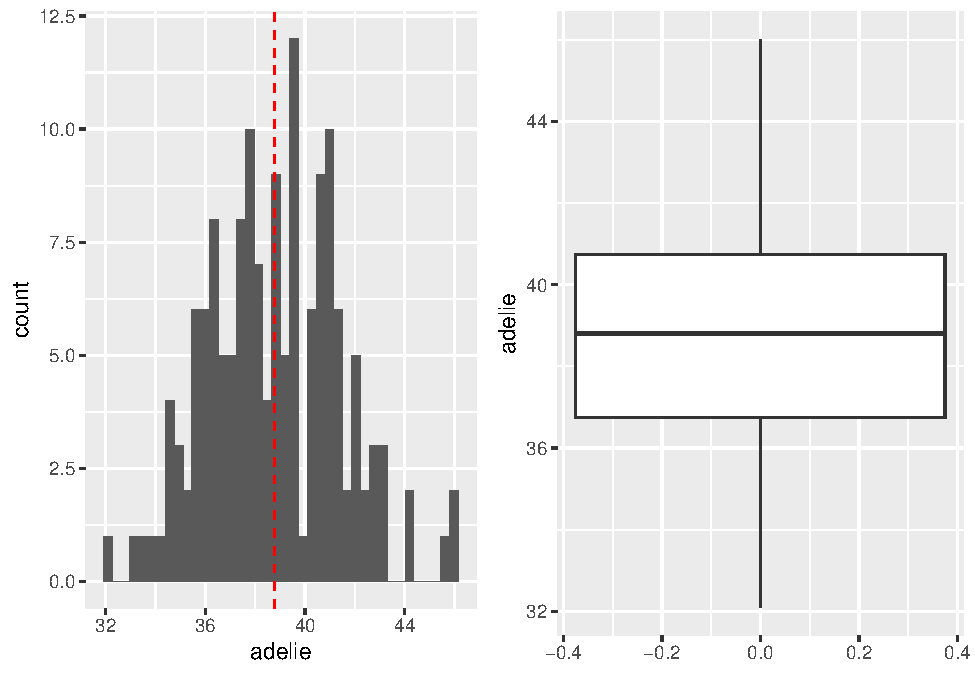
\includegraphics{Tests_and_Applications_files/figure-latex/unnamed-chunk-5-1.pdf}
The distribution of \texttt{adelie} seems symmetric around the mean and
the median, and unimodal. From the boxplot no outliers are clearly
visible. Additionally, we can compare the sample quantiles with the
quantiles of the normal distribution.

\begin{Shaded}
\begin{Highlighting}[]
\FunctionTok{qqnorm}\NormalTok{(adelie, }\AttributeTok{plot.it =} \ConstantTok{TRUE}\NormalTok{)}
\FunctionTok{qqline}\NormalTok{(adelie, }\AttributeTok{col=}\StringTok{"red"}\NormalTok{)}
\end{Highlighting}
\end{Shaded}

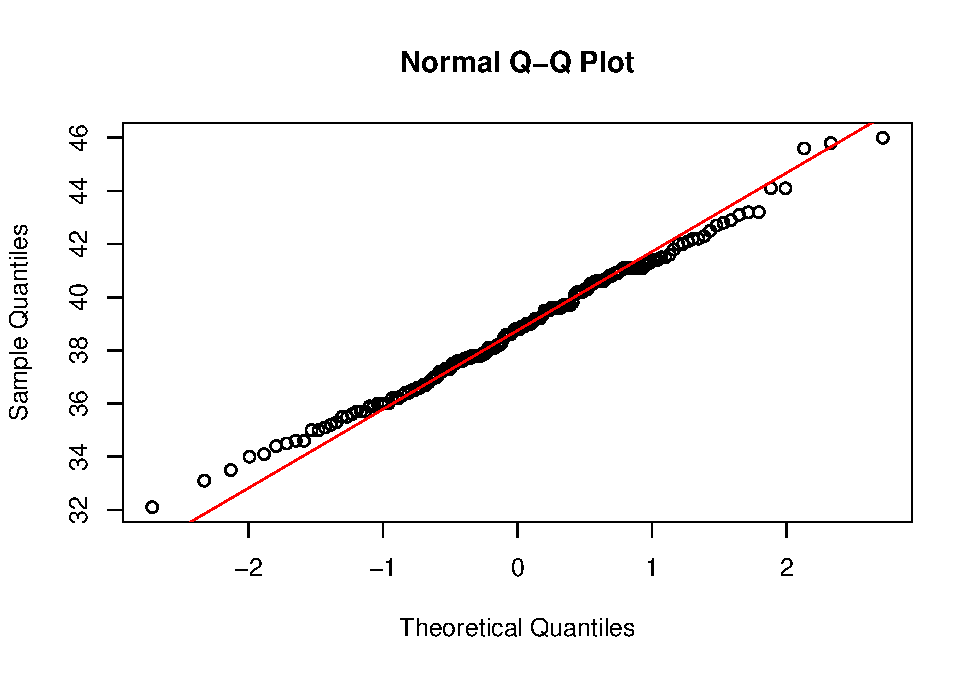
\includegraphics{Tests_and_Applications_files/figure-latex/unnamed-chunk-6-1.pdf}

\begin{Shaded}
\begin{Highlighting}[]
\FunctionTok{ggplot}\NormalTok{(}\AttributeTok{mapping =} \FunctionTok{aes}\NormalTok{(}\AttributeTok{sample=}\NormalTok{adelie)) }\SpecialCharTok{+} 
  \FunctionTok{geom\_qq}\NormalTok{()}\SpecialCharTok{+}
  \FunctionTok{geom\_qq\_line}\NormalTok{(}\AttributeTok{color=}\StringTok{"red"}\NormalTok{)}
\end{Highlighting}
\end{Shaded}

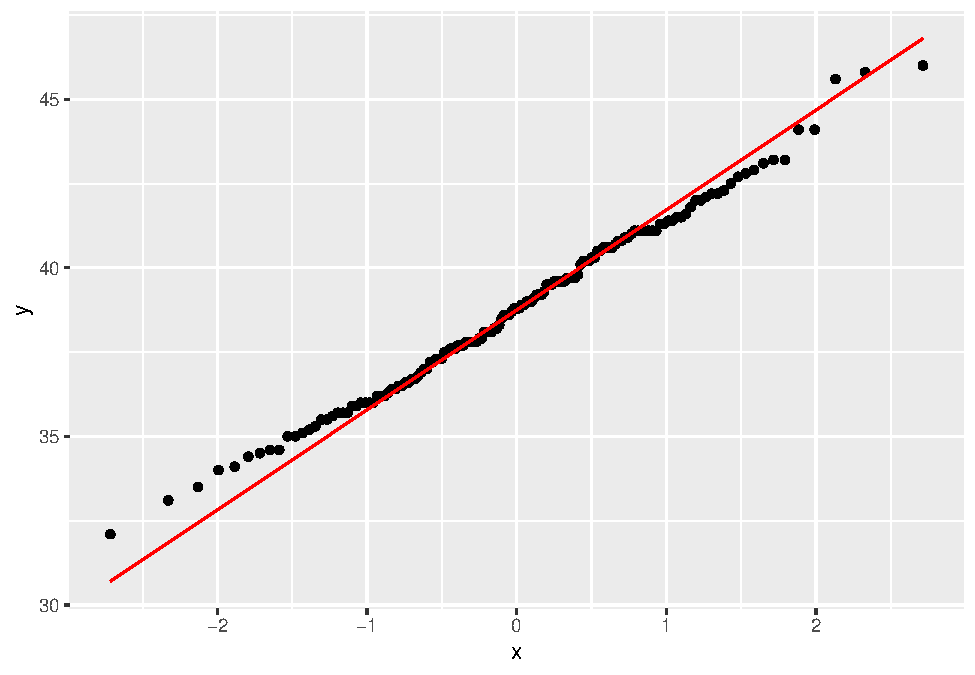
\includegraphics{Tests_and_Applications_files/figure-latex/unnamed-chunk-7-1.pdf}
We have added the line of theoretical quantile-quantile plot. The data
is approximately normal, as the points largely follow the qqline. There
are minor deviations at the tails and there are no extreme points
(outliers) far away from the line. Finally, we can also perform a
statistical test with null hypothesus \(H_0\): the sample follows a
normal distribution. Testing is data points followsì a specific
distribution is referred to as \emph{Goodness-of-fit} testing. One of
the most used method for testing normality is the \emph{Shapiro-Wilk}
test.

\begin{Shaded}
\begin{Highlighting}[]
\FunctionTok{shapiro.test}\NormalTok{(adelie)}
\end{Highlighting}
\end{Shaded}

\begin{verbatim}
## 
##  Shapiro-Wilk normality test
## 
## data:  adelie
## W = 0.99336, p-value = 0.7166
\end{verbatim}

The obtained p-value corroborates the previous conclusions.

\begin{quote}
Test for normality shoul be used with caution. A low sample size could
not provide enough evidence for rejecting the null hypothesis, even if
data are not normally distributed. On the other side, a very large
sample size can reject the null hypothesis even in the cases where the
deviation from the normal distribution is not so large.
\end{quote}

We can do the same for the \texttt{gentoo} sample.

\begin{Shaded}
\begin{Highlighting}[]
\NormalTok{p1 }\OtherTok{\textless{}{-}} \FunctionTok{ggplot}\NormalTok{(}\AttributeTok{mapping=} \FunctionTok{aes}\NormalTok{(}\AttributeTok{x=}\NormalTok{gentoo))}\SpecialCharTok{+}
  \FunctionTok{geom\_histogram}\NormalTok{(}\AttributeTok{bins =} \DecValTok{40}\NormalTok{) }\SpecialCharTok{+} 
  \FunctionTok{geom\_vline}\NormalTok{(}\AttributeTok{xintercept =}\NormalTok{ mu\_g, }\AttributeTok{color=}\StringTok{"red"}\NormalTok{, }\AttributeTok{linetype=}\StringTok{"dashed"}\NormalTok{)}
\NormalTok{p2 }\OtherTok{\textless{}{-}} \FunctionTok{ggplot}\NormalTok{(}\AttributeTok{mapping=} \FunctionTok{aes}\NormalTok{(}\AttributeTok{y=}\NormalTok{gentoo))}\SpecialCharTok{+}
  \FunctionTok{geom\_boxplot}\NormalTok{(}\AttributeTok{outliers =} \ConstantTok{TRUE}\NormalTok{)}
\NormalTok{gridExtra}\SpecialCharTok{::}\FunctionTok{grid.arrange}\NormalTok{(p1, p2, }\AttributeTok{nrow=}\DecValTok{1}\NormalTok{)}
\end{Highlighting}
\end{Shaded}

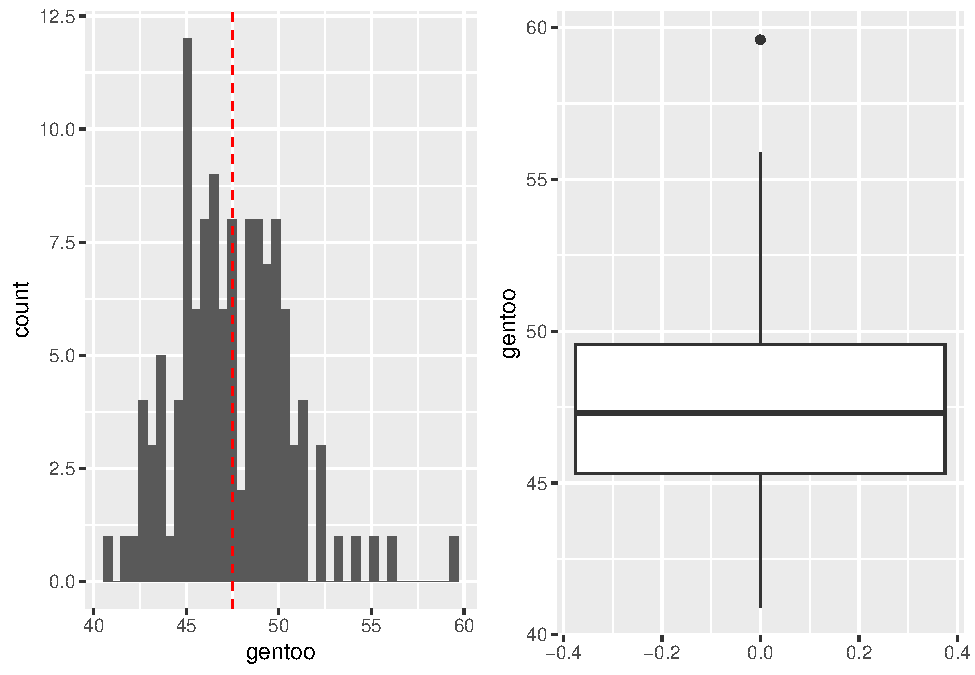
\includegraphics{Tests_and_Applications_files/figure-latex/unnamed-chunk-9-1.pdf}
The distribution of \texttt{gentoo} seems symmetric around the mean and
the median, and unimodal. From the boxplot one outlier is displayed on
the right tail of the distribution. The havier right tail is also
suggested by the histogram. Additionally, we compare the sample
quantiles with the quantiles of the normal distribution.

\begin{Shaded}
\begin{Highlighting}[]
\FunctionTok{qqnorm}\NormalTok{(gentoo, }\AttributeTok{plot.it =} \ConstantTok{TRUE}\NormalTok{)}
\FunctionTok{qqline}\NormalTok{(gentoo, }\AttributeTok{col=}\StringTok{"red"}\NormalTok{)}
\end{Highlighting}
\end{Shaded}

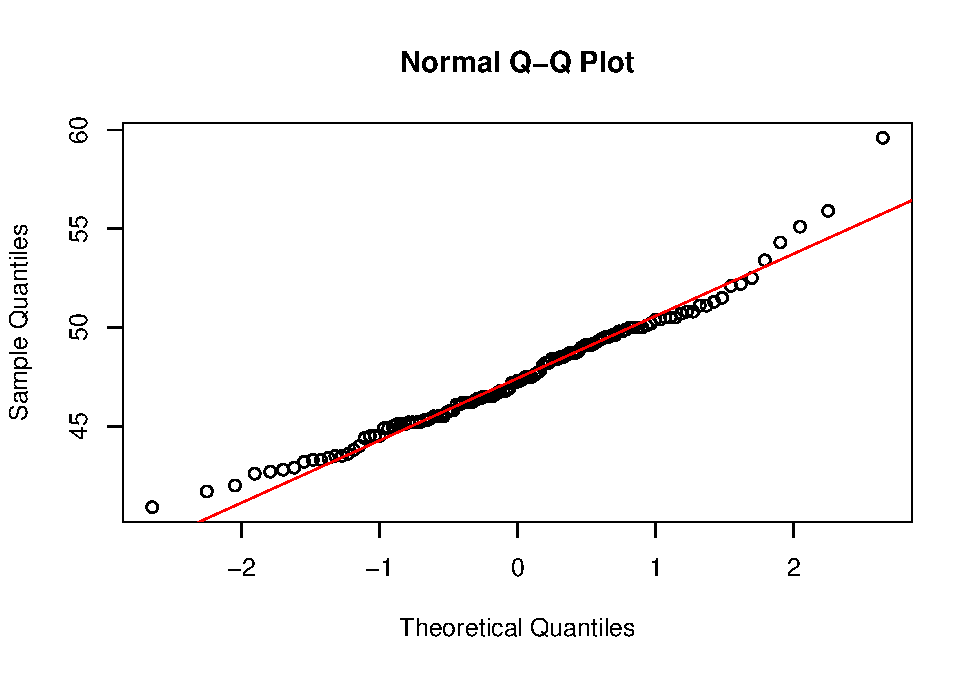
\includegraphics{Tests_and_Applications_files/figure-latex/unnamed-chunk-10-1.pdf}

\begin{Shaded}
\begin{Highlighting}[]
\FunctionTok{ggplot}\NormalTok{(}\AttributeTok{mapping =} \FunctionTok{aes}\NormalTok{(}\AttributeTok{sample=}\NormalTok{gentoo)) }\SpecialCharTok{+} 
  \FunctionTok{geom\_qq}\NormalTok{()}\SpecialCharTok{+}
  \FunctionTok{geom\_qq\_line}\NormalTok{(}\AttributeTok{color=}\StringTok{"red"}\NormalTok{)}
\end{Highlighting}
\end{Shaded}

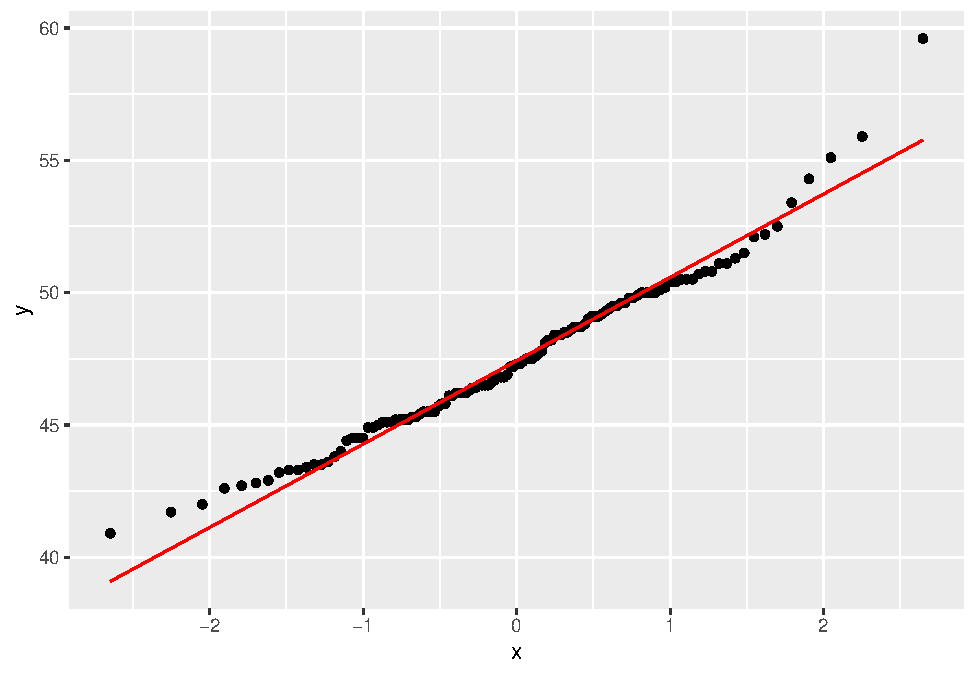
\includegraphics{Tests_and_Applications_files/figure-latex/unnamed-chunk-11-1.pdf}
The deviations in the tails suggest that the data has heavier tails. The
extreme deviations on both ends could be indicative of outliers or
values that are unusually large/small relative to what is expected under
normality. Finally, we can also perform the Shapiro-Wilk test.

\begin{Shaded}
\begin{Highlighting}[]
\FunctionTok{shapiro.test}\NormalTok{(gentoo)}
\end{Highlighting}
\end{Shaded}

\begin{verbatim}
## 
##  Shapiro-Wilk normality test
## 
## data:  gentoo
## W = 0.97272, p-value = 0.01349
\end{verbatim}

Considering the 0.05 confidence level used for computing the test, the
obtained p-value corroborates the previous conclusions, suggesting to
reject the null hypothesis. Notice that, if we remove the outlying
oservation, the sample is more likely following a normal distribution.

\begin{Shaded}
\begin{Highlighting}[]
\NormalTok{gentoo0 }\OtherTok{\textless{}{-}}\NormalTok{ gentoo[}\SpecialCharTok{{-}}\FunctionTok{which.max}\NormalTok{(gentoo)]}
\FunctionTok{ggplot}\NormalTok{(}\AttributeTok{mapping =} \FunctionTok{aes}\NormalTok{(}\AttributeTok{sample=}\NormalTok{gentoo0)) }\SpecialCharTok{+} 
  \FunctionTok{geom\_qq}\NormalTok{()}\SpecialCharTok{+}
  \FunctionTok{geom\_qq\_line}\NormalTok{(}\AttributeTok{color=}\StringTok{"red"}\NormalTok{)}
\end{Highlighting}
\end{Shaded}

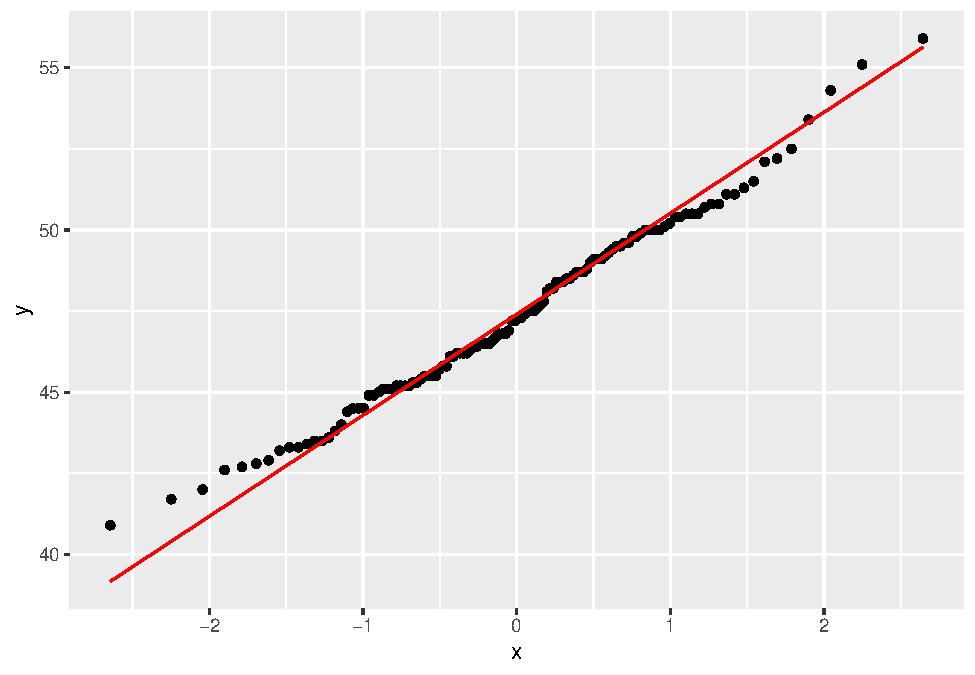
\includegraphics{Tests_and_Applications_files/figure-latex/unnamed-chunk-13-1.pdf}

\begin{Shaded}
\begin{Highlighting}[]
\FunctionTok{shapiro.test}\NormalTok{(gentoo0)}
\end{Highlighting}
\end{Shaded}

\begin{verbatim}
## 
##  Shapiro-Wilk normality test
## 
## data:  gentoo0
## W = 0.98862, p-value = 0.4068
\end{verbatim}

Finally, we apply the t.test for comparing their mean

\begin{Shaded}
\begin{Highlighting}[]
\FunctionTok{t.test}\NormalTok{(adelie, gentoo, }\AttributeTok{var.equal =} \ConstantTok{TRUE}\NormalTok{, }\AttributeTok{paired =} \ConstantTok{FALSE}\NormalTok{)}
\end{Highlighting}
\end{Shaded}

\begin{verbatim}
## 
##  Two Sample t-test
## 
## data:  adelie and gentoo
## t = -25.095, df = 272, p-value < 2.2e-16
## alternative hypothesis: true difference in means is not equal to 0
## 95 percent confidence interval:
##  -9.397060 -8.029915
## sample estimates:
## mean of x mean of y 
##  38.79139  47.50488
\end{verbatim}

Here, the difference between is clearly different from zero and this
difference is statistically significant. In this case, the presence of
the outlier does not affect the result.

\hypertarget{transformations-of-data}{%
\subsubsection{Transformations of data}\label{transformations-of-data}}

One possible technique is to transform data points to improve the
goodness of fit to the assumed distribution. Notice that it is not a
good idea to try several transformations for findng the one that has the
best fit with the model assumptions.

\hypertarget{non-parametric-approach}{%
\subsubsection{Non-parametric approach}\label{non-parametric-approach}}

In case of violations of the model assumption, we can use non-parametric
tests, which have less assumptions on the distributions of the
variables. For example the \emph{permutation-based test} (with the
function \texttt{independence\_test} from the \texttt{coin} package) and
the \emph{sign test} are alternatives to the t.test for the mean.\\
When we want to compare two means and the normality assumptions are not
satisfied, we can use the \emph{Mann-Whitney \(U\) test} which only
assumes independent samples.

\begin{Shaded}
\begin{Highlighting}[]
\FunctionTok{wilcox.test}\NormalTok{(adelie, gentoo)}
\end{Highlighting}
\end{Shaded}

\begin{verbatim}
## 
##  Wilcoxon rank sum test with continuity correction
## 
## data:  adelie and gentoo
## W = 224.5, p-value < 2.2e-16
## alternative hypothesis: true location shift is not equal to 0
\end{verbatim}

\hypertarget{robust-statistics}{%
\subsubsection{Robust statistics}\label{robust-statistics}}

We have seen that assumptions are often violated due to the presence of
non-normality or outliers and then tests canbecome unreliable. To
address these limitations, robust alternatives have been developed in
order to provide more accurate p-values and confidence intervals while
being less sensitive to violations of model assumptions. Notice that
non-parametric tests, even if not explicitly robust, offer alternatives
that avoid the need for normality assumptions.

For comparing the means of two groups we can use the \emph{Yuen's
trimmed-mean test} (trims a percentage of extreme values from both tails
before performing a t-test)

\begin{Shaded}
\begin{Highlighting}[]
\FunctionTok{library}\NormalTok{(WRS2)}
\end{Highlighting}
\end{Shaded}

\begin{verbatim}
## Warning: il pacchetto 'WRS2' è stato creato con R versione 4.3.3
\end{verbatim}

\begin{Shaded}
\begin{Highlighting}[]
\NormalTok{dat }\OtherTok{\textless{}{-}} \FunctionTok{data.frame}\NormalTok{(}\AttributeTok{bill\_length =} \FunctionTok{c}\NormalTok{(adelie,gentoo), }\AttributeTok{species =}\FunctionTok{rep}\NormalTok{(}\FunctionTok{c}\NormalTok{(}\DecValTok{1}\NormalTok{,}\DecValTok{0}\NormalTok{),}\AttributeTok{times=}\FunctionTok{c}\NormalTok{(}\DecValTok{151}\NormalTok{,}\DecValTok{123}\NormalTok{)))}
\FunctionTok{yuen}\NormalTok{(bill\_length }\SpecialCharTok{\textasciitilde{}}\NormalTok{ species,}\AttributeTok{data =}\NormalTok{  dat, }\AttributeTok{tr =} \FloatTok{0.2}\NormalTok{) }\CommentTok{\# tr = trimming percentage}
\end{Highlighting}
\end{Shaded}

\begin{verbatim}
## Call:
## yuen(formula = bill_length ~ species, data = dat, tr = 0.2)
## 
## Test statistic: 22.6846 (df = 154.36), p-value = 0
## 
## Trimmed mean difference:  8.60983 
## 95 percent confidence interval:
## 7.8601     9.3596 
## 
## Explanatory measure of effect size: 0.96
\end{verbatim}

or the \emph{permutation test}.

\begin{Shaded}
\begin{Highlighting}[]
\NormalTok{coin}\SpecialCharTok{::}\FunctionTok{independence\_test}\NormalTok{(bill\_length }\SpecialCharTok{\textasciitilde{}}\NormalTok{ species, dat)}
\end{Highlighting}
\end{Shaded}

\begin{verbatim}
## 
##  Asymptotic General Independence Test
## 
## data:  bill_length by species
## Z = -13.808, p-value < 2.2e-16
## alternative hypothesis: two.sided
\end{verbatim}

\hypertarget{how-to-choose-the-appropriate-test}{%
\subsubsection{How to choose the appropriate
test?}\label{how-to-choose-the-appropriate-test}}

The tests used along these notes are not intended to be the suggested
ones in practice. Mostly are the firstly introduced methods in
statistical hypothesis testing and are considered here to show the
reasoning behind the translation of the research question to a null
hypothesis and how the confidence intervals and statistical tests can
help in making some statistically significant inference on the data. ~
In order to choose the appropriate test to use in our analysis, it is
important to consider the following steps.

\begin{itemize}
\tightlist
\item
  Use the graphical methods introduced in the Exploratory analysis
  section in order to \emph{know} your data.
\end{itemize}

\begin{longtable}[]{@{}ll@{}}
\toprule\noalign{}
\textbf{Type of data} & \textbf{graphical method} \\
\midrule\noalign{}
\endhead
\bottomrule\noalign{}
\endlastfoot
Categorical & barplot \\
Numerical & Histogram \\
& boxplot \\
& density \\
Two Categorical & Grouped Barplot \\
& Contingency table \\
One Numerical and one categorical & Grouped Histograms \\
& Grouped Boxplots \\
Two Numerical & Scatter plot \\
& Line plot \\
\end{longtable}

\begin{itemize}
\tightlist
\item
  Are you studying a single variable or the association of two or more
  variables?
\item
  The considered variables are Categorical or Numerical?
\item
  What is the research question that we are investigating? It is crucial
  to define the correct null hypothesis for understanding the
  appropriate tests.
\item
  What are the assumptions of the available tests? The assumptions of
  the method must be satisfied by our data to obtain reliable results.
\item
  Search the literature for the most innovative procedures that show the
  best fit with the complexities in the data in hand. Do not limit
  yourself to the use of standard and well-known methods. In the
  statistical literature, new methods are developed to address specific
  situations, to be robust against model mispecifications or overcome
  sources of errors in specific applications. Know the performance in
  terms of level (significance level \(\alpha\)) and power of the test
  in different situations.
\end{itemize}

\hypertarget{analysis-of-variance-anova}{%
\subsection{Analysis of Variance
(ANOVA)}\label{analysis-of-variance-anova}}

In this section, we consider the case where we have two random
variables, \(X\) and \(Y\), where one of them, say \(X\) is qualitative.
In this case, we want to compare the conditional distributions, or in
other words we want to verify if observations (\(Y\)) in different
groups (levels of \(X\)) are different on average. The Analysis of
Variance, or ANOVA, is the most famous tool for evaluating
simultaneously the equality of means of \(k\) groups. In general, we say
that \(Y\) is independent on average from \(X\) when \(X\) does not
influence the mean of \(Y\). Hence, we test \[
\begin{cases}
H_0 &: \mu_1 = \ldots = \mu_k \\ 
H_1 &: \text{at least one }\mu_i\text{ is different from the others}
\end{cases}
\]

Let us consider the following example.\\
To determine whether and to what extent the type of meat used to prepare
hot dogs influences their calorie content, the calories of 54 packages
from different brands were measured. These data are stored in the data
frame hot\_dog:

\begin{Shaded}
\begin{Highlighting}[]
\FunctionTok{load}\NormalTok{(}\StringTok{"hotdog.Rdata"}\NormalTok{)}
\FunctionTok{colnames}\NormalTok{(hot\_dog) }\OtherTok{\textless{}{-}} \FunctionTok{c}\NormalTok{(}\StringTok{"meat"}\NormalTok{, }\StringTok{"calories"}\NormalTok{)}
\FunctionTok{summary}\NormalTok{(hot\_dog)}
\end{Highlighting}
\end{Shaded}

\begin{verbatim}
##       meat       calories    
##  Bovina :20   Min.   : 86.0  
##  Mista  :17   1st Qu.:132.0  
##  Pollame:17   Median :145.0  
##               Mean   :145.4  
##               3rd Qu.:172.8  
##               Max.   :195.0
\end{verbatim}

First, we compute the main descriptive statistics and represent the
distributions, based on the type of meat, using boxplots. In this
dataset, we have a single numeric vector, calories, whose elements are
grouped according to the levels of the factor variable meat. We can use
the by function, specifying the numeric vector, the grouping factor, and
the operation to apply. For example

\begin{Shaded}
\begin{Highlighting}[]
\FunctionTok{attach}\NormalTok{(hot\_dog)}
\NormalTok{group\_sizes }\OtherTok{\textless{}{-}} \FunctionTok{by}\NormalTok{(calories, meat, length)}
\NormalTok{n }\OtherTok{\textless{}{-}} \FunctionTok{sum}\NormalTok{(group\_sizes)}
\NormalTok{sigma2 }\OtherTok{\textless{}{-}} \ControlFlowTok{function}\NormalTok{(x)\{}
\NormalTok{  v }\OtherTok{\textless{}{-}} \FunctionTok{mean}\NormalTok{((x }\SpecialCharTok{{-}} \FunctionTok{mean}\NormalTok{(x))}\SpecialCharTok{\^{}}\DecValTok{2}\NormalTok{)}
  \FunctionTok{return}\NormalTok{(v)}
\NormalTok{\}}
\NormalTok{means }\OtherTok{\textless{}{-}} \FunctionTok{by}\NormalTok{(calories, meat, mean)}
\NormalTok{variances }\OtherTok{\textless{}{-}} \FunctionTok{by}\NormalTok{(calories, meat, sigma2)}
\FunctionTok{print}\NormalTok{(}\FunctionTok{cbind}\NormalTok{(means, variances))}
\end{Highlighting}
\end{Shaded}

\begin{verbatim}
##            means variances
## Bovina  156.8500  487.0275
## Mista   158.7059  599.3841
## Pollame 118.7647  478.6505
\end{verbatim}

The overall mean and variance are

\begin{Shaded}
\begin{Highlighting}[]
\NormalTok{mu }\OtherTok{\textless{}{-}} \FunctionTok{mean}\NormalTok{(calories)}
\NormalTok{v }\OtherTok{\textless{}{-}} \FunctionTok{sigma2}\NormalTok{(calories)}
\FunctionTok{print}\NormalTok{(}\FunctionTok{c}\NormalTok{(mu, v))}
\end{Highlighting}
\end{Shaded}

\begin{verbatim}
## [1] 145.4444 847.3951
\end{verbatim}

The total number of groups \(k\) is

\begin{Shaded}
\begin{Highlighting}[]
\NormalTok{k }\OtherTok{\textless{}{-}} \FunctionTok{length}\NormalTok{(}\FunctionTok{levels}\NormalTok{(meat))}
\NormalTok{k}
\end{Highlighting}
\end{Shaded}

\begin{verbatim}
## [1] 3
\end{verbatim}

\begin{Shaded}
\begin{Highlighting}[]
\FunctionTok{detach}\NormalTok{(hot\_dog)}
\end{Highlighting}
\end{Shaded}

The boxplot for calorie distributions by meat type can be plotted using

\begin{Shaded}
\begin{Highlighting}[]
\FunctionTok{boxplot}\NormalTok{(calories }\SpecialCharTok{\textasciitilde{}}\NormalTok{ meat, hot\_dog)}
\end{Highlighting}
\end{Shaded}

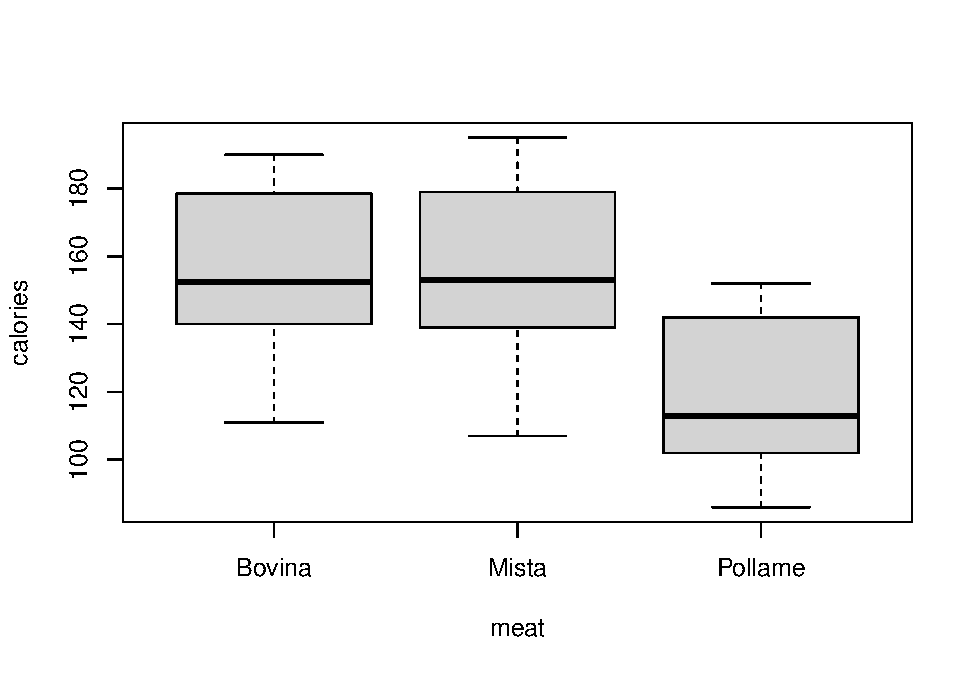
\includegraphics{Tests_and_Applications_files/figure-latex/unnamed-chunk-22-1.pdf}

\begin{Shaded}
\begin{Highlighting}[]
\FunctionTok{ggplot}\NormalTok{(hot\_dog, }\FunctionTok{aes}\NormalTok{(}\AttributeTok{x=}\NormalTok{meat,}\AttributeTok{y=}\NormalTok{calories,}\AttributeTok{fill=}\NormalTok{meat))}\SpecialCharTok{+}
  \FunctionTok{geom\_boxplot}\NormalTok{()}
\end{Highlighting}
\end{Shaded}

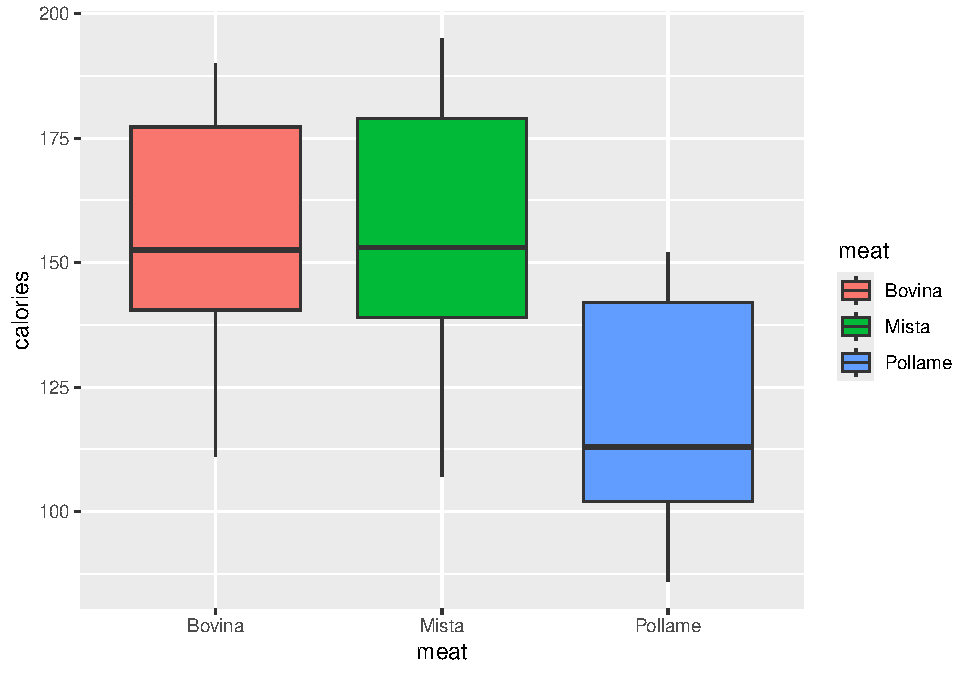
\includegraphics{Tests_and_Applications_files/figure-latex/unnamed-chunk-22-2.pdf}

Note that the custom function \texttt{sigma2} computes the variance as
the mean of squared deviations (dividing by \(n\), not \(n-1\) as in the
sample variance). The values and the plot suggest a clear difference for
the third group (Poultry). To test if this difference is significant, we
conduct a hypothesis test with \(H_0: \mu_1 = \mu_2 = \mu_3\).

We compute the sum of squared deviations from the group means (SS error)
and the sum of squared deviations of group means from the overall mean
(SS groups) \[
  SS_{\text{err}} = \frac{1}{n} \sum_{i=1}^k \sum_{j=1}^{n_i} (x_{ij} - \mu_i)^2, \quad 
  SS_{\text{groups}} = \frac{1}{n} \sum_{i=1}^k n_i (\mu_i - \mu)^2
  \]

\begin{Shaded}
\begin{Highlighting}[]
\NormalTok{sse }\OtherTok{\textless{}{-}} \FunctionTok{sum}\NormalTok{(group\_sizes }\SpecialCharTok{*}\NormalTok{ variances)}
\NormalTok{ssg }\OtherTok{\textless{}{-}} \FunctionTok{sum}\NormalTok{(group\_sizes }\SpecialCharTok{*}\NormalTok{ (means }\SpecialCharTok{{-}}\NormalTok{ mu)}\SpecialCharTok{\^{}}\DecValTok{2}\NormalTok{)}
\FunctionTok{print}\NormalTok{(}\FunctionTok{c}\NormalTok{(ssg, sse))}
\end{Highlighting}
\end{Shaded}

\begin{verbatim}
## [1] 17692.20 28067.14
\end{verbatim}

\hypertarget{variance-decomposition}{%
\paragraph{Variance Decomposition}\label{variance-decomposition}}

These two quantities are also known as within-group variance (SS error)
and between-group variance ( SS groups). Note that \[
  \frac{SS_{\text{err}}}{n} + \frac{SS_{\text{groups}}}{n} = S^2
  \]

where \(S^2\) is the total variance of all observations with respect to
the overall mean.

\begin{Shaded}
\begin{Highlighting}[]
\FunctionTok{print}\NormalTok{(}\FunctionTok{c}\NormalTok{(sse}\SpecialCharTok{/}\NormalTok{n }\SpecialCharTok{+}\NormalTok{ ssg}\SpecialCharTok{/}\NormalTok{n, v))}
\end{Highlighting}
\end{Shaded}

\begin{verbatim}
## [1] 847.3951 847.3951
\end{verbatim}

This result shows that dividing the data into groups explains part of
the variability. Specifically, the total variance can be decomposed into
a portion that describes differences between group means and a portion
describing differences within groups.

\hypertarget{pearson-correlation-ratio}{%
\paragraph{Pearson Correlation Ratio}\label{pearson-correlation-ratio}}

Using these quantities, we can calculate the Pearson correlation ratio

\begin{Shaded}
\begin{Highlighting}[]
\NormalTok{eta2 }\OtherTok{\textless{}{-}}\NormalTok{ (ssg }\SpecialCharTok{/}\NormalTok{ n) }\SpecialCharTok{/}\NormalTok{ v}
\NormalTok{eta2}
\end{Highlighting}
\end{Shaded}

\begin{verbatim}
## [1] 0.3866358
\end{verbatim}

In general, it ranges between 0 and 1, where 0 indicates independence
(the mean does not depend on grouping), and 1 indicates perfect
dependence.

Normalizing the sums, we compute \[
  MS_{\text{err}} = \frac{SS_{\text{err}}}{n - k}, \quad MS_{\text{groups}} = \frac{SS_{\text{groups}}}{k - 1}.
  \] Then, the test statistic is
\[F=\frac{MS_{\text{groups}}}{MS_{\text{err}}}.\] Under \(H_0\) this
follows an \(F\)-distribution with \(k-1\) and \(n-k\) degrees of
freedom. We reject \(H_0\) if the observed \(F\)-value exceeds the
\((1-\alpha)\)-quantile of the \(F\)-distribution for \(\alpha=0.05\).

\begin{Shaded}
\begin{Highlighting}[]
\NormalTok{alpha }\OtherTok{\textless{}{-}} \FloatTok{0.05}
\NormalTok{msg }\OtherTok{\textless{}{-}}\NormalTok{ ssg }\SpecialCharTok{/}\NormalTok{ (k }\SpecialCharTok{{-}} \DecValTok{1}\NormalTok{)}
\NormalTok{mse }\OtherTok{\textless{}{-}}\NormalTok{ sse }\SpecialCharTok{/}\NormalTok{ (n }\SpecialCharTok{{-}}\NormalTok{ k)}
\FunctionTok{print}\NormalTok{(}\FunctionTok{c}\NormalTok{(msg, mse))}
\end{Highlighting}
\end{Shaded}

\begin{verbatim}
## [1] 8846.098  550.336
\end{verbatim}

\begin{Shaded}
\begin{Highlighting}[]
\NormalTok{f\_oss }\OtherTok{\textless{}{-}}\NormalTok{ msg }\SpecialCharTok{/}\NormalTok{ mse}
\FunctionTok{pf}\NormalTok{(f\_oss, k }\SpecialCharTok{{-}} \DecValTok{1}\NormalTok{, n }\SpecialCharTok{{-}}\NormalTok{ k, }\AttributeTok{lower.tail =} \ConstantTok{FALSE}\NormalTok{)}
\end{Highlighting}
\end{Shaded}

\begin{verbatim}
## [1] 3.862072e-06
\end{verbatim}

In R, ANOVA can be performed directly using the \texttt{aov} function:

\begin{Shaded}
\begin{Highlighting}[]
\NormalTok{model }\OtherTok{\textless{}{-}} \FunctionTok{aov}\NormalTok{(calories }\SpecialCharTok{\textasciitilde{}}\NormalTok{ meat, hot\_dog)}
\NormalTok{model}
\end{Highlighting}
\end{Shaded}

\begin{verbatim}
## Call:
##    aov(formula = calories ~ meat, data = hot_dog)
## 
## Terms:
##                     meat Residuals
## Sum of Squares  17692.19  28067.14
## Deg. of Freedom        2        51
## 
## Residual standard error: 23.45924
## Estimated effects may be unbalanced
\end{verbatim}

\begin{Shaded}
\begin{Highlighting}[]
\FunctionTok{summary}\NormalTok{(model)}
\end{Highlighting}
\end{Shaded}

\begin{verbatim}
##             Df Sum Sq Mean Sq F value   Pr(>F)    
## meat         2  17692    8846   16.07 3.86e-06 ***
## Residuals   51  28067     550                     
## ---
## Signif. codes:  0 '***' 0.001 '**' 0.01 '*' 0.05 '.' 0.1 ' ' 1
\end{verbatim}

For the \(F\)-test results, use

\begin{Shaded}
\begin{Highlighting}[]
\FunctionTok{anova}\NormalTok{(model)}
\end{Highlighting}
\end{Shaded}

\begin{verbatim}
## Analysis of Variance Table
## 
## Response: calories
##           Df Sum Sq Mean Sq F value    Pr(>F)    
## meat       2  17692  8846.1  16.074 3.862e-06 ***
## Residuals 51  28067   550.3                      
## ---
## Signif. codes:  0 '***' 0.001 '**' 0.01 '*' 0.05 '.' 0.1 ' ' 1
\end{verbatim}

In practice, the \texttt{aov} function is a special case of the
\texttt{lm} function, which can be used in the same way.

\begin{Shaded}
\begin{Highlighting}[]
\FunctionTok{attach}\NormalTok{(hot\_dog)}
\NormalTok{modello2 }\OtherTok{\textless{}{-}} \FunctionTok{lm}\NormalTok{(calories }\SpecialCharTok{\textasciitilde{}}\NormalTok{ meat, hot\_dog)}
\FunctionTok{anova}\NormalTok{(modello2)}
\end{Highlighting}
\end{Shaded}

\begin{verbatim}
## Analysis of Variance Table
## 
## Response: calories
##           Df Sum Sq Mean Sq F value    Pr(>F)    
## meat       2  17692  8846.1  16.074 3.862e-06 ***
## Residuals 51  28067   550.3                      
## ---
## Signif. codes:  0 '***' 0.001 '**' 0.01 '*' 0.05 '.' 0.1 ' ' 1
\end{verbatim}

Using the \texttt{anova} function, we obtain the same results, but the
\texttt{modello2} object contains more information. If the test
indicates that there is a difference between groups, we are naturally
interested in identifying where this difference lies. For this purpose,
pairwise comparisons between the groups are useful. These can be
extracted using the \texttt{summary} function

\begin{Shaded}
\begin{Highlighting}[]
\FunctionTok{summary}\NormalTok{(modello2)}
\end{Highlighting}
\end{Shaded}

\begin{verbatim}
## 
## Call:
## lm(formula = calories ~ meat, data = hot_dog)
## 
## Residuals:
##     Min      1Q  Median      3Q     Max 
## -51.706 -18.492  -5.278  22.500  36.294 
## 
## Coefficients:
##             Estimate Std. Error t value Pr(>|t|)    
## (Intercept)  156.850      5.246  29.901  < 2e-16 ***
## meatMista      1.856      7.739   0.240    0.811    
## meatPollame  -38.085      7.739  -4.921 9.39e-06 ***
## ---
## Signif. codes:  0 '***' 0.001 '**' 0.01 '*' 0.05 '.' 0.1 ' ' 1
## 
## Residual standard error: 23.46 on 51 degrees of freedom
## Multiple R-squared:  0.3866, Adjusted R-squared:  0.3626 
## F-statistic: 16.07 on 2 and 51 DF,  p-value: 3.862e-06
\end{verbatim}

The aspect of multiple comparisons is not treated here.

A non parametric alternative is the \emph{Kruskal-Wallis test} with the
assumption that the distribution of the variable must be the same in
each population.

\begin{Shaded}
\begin{Highlighting}[]
\FunctionTok{kruskal.test}\NormalTok{(calories}\SpecialCharTok{\textasciitilde{}}\NormalTok{meat, hot\_dog)}
\end{Highlighting}
\end{Shaded}

\begin{verbatim}
## 
##  Kruskal-Wallis rank sum test
## 
## data:  calories by meat
## Kruskal-Wallis chi-squared = 19.251, df = 2, p-value = 6.601e-05
\end{verbatim}

\hypertarget{hypothesis-verification}{%
\subsubsection{Hypothesis Verification}\label{hypothesis-verification}}

The ANOVA test assumes that the variable is normally distributed in each
of the \(k\) populations and the variance is the same in all the
populations. So it is important to verify whether this assumption holds.
Since we do not know the true variances of each group, we can perform a
test to determine (with a given confidence level) whether the assumption
is satisfied. For this, Bartlett's test can be used, where the null
hypothesis corresponds to the equality of variances

\begin{Shaded}
\begin{Highlighting}[]
\FunctionTok{bartlett.test}\NormalTok{(calories}\SpecialCharTok{\textasciitilde{}}\NormalTok{meat)}
\end{Highlighting}
\end{Shaded}

\begin{verbatim}
## 
##  Bartlett test of homogeneity of variances
## 
## data:  calories by meat
## Bartlett's K-squared = 0.26732, df = 2, p-value = 0.8749
\end{verbatim}

\begin{Shaded}
\begin{Highlighting}[]
\FunctionTok{detach}\NormalTok{(hot\_dog)}
\end{Highlighting}
\end{Shaded}

\textbf{Note}: It is crucial to verify that the assumptions hold for the
given study. Otherwise, the test results are meaningless!

\hypertarget{correlation-and-regression-analysis}{%
\subsection{Correlation and Regression
Analysis}\label{correlation-and-regression-analysis}}

In this section, we consider situations where we want to describe the
relationship between two continuous variables.

Let \(X\) and \(Y\) be two continuous random variables with samples
\((x_1, \ldots, x_n)\) and \((y_1, \ldots, y_n)\), respectively. To
assess the relationship between these two variables, we can start with a
scatter plot, which displays the points \((x_i, y_i)\) on a Cartesian
plane. Consider the following example:

A real estate agent wants to predict the monthly rent of apartments
based on their size. For this purpose, they conduct a survey and collect
data on 25 apartments in a residential area (rent in dollars, size in
square feet).

\begin{Shaded}
\begin{Highlighting}[]
\NormalTok{data }\OtherTok{\textless{}{-}} \FunctionTok{data.frame}\NormalTok{(}
  \AttributeTok{rent =} \FunctionTok{c}\NormalTok{(}\DecValTok{950}\NormalTok{, }\DecValTok{1600}\NormalTok{, }\DecValTok{1200}\NormalTok{, }\DecValTok{1500}\NormalTok{, }\DecValTok{950}\NormalTok{, }\DecValTok{1700}\NormalTok{, }\DecValTok{1650}\NormalTok{, }\DecValTok{935}\NormalTok{, }\DecValTok{875}\NormalTok{, }\DecValTok{1150}\NormalTok{, }\DecValTok{1400}\NormalTok{, }\DecValTok{1650}\NormalTok{, }
           \DecValTok{2300}\NormalTok{, }\DecValTok{1800}\NormalTok{, }\DecValTok{1400}\NormalTok{, }\DecValTok{1450}\NormalTok{, }\DecValTok{1100}\NormalTok{, }\DecValTok{1700}\NormalTok{, }\DecValTok{1200}\NormalTok{, }\DecValTok{1150}\NormalTok{, }\DecValTok{1600}\NormalTok{, }\DecValTok{1650}\NormalTok{, }\DecValTok{1200}\NormalTok{, }
           \DecValTok{800}\NormalTok{, }\DecValTok{1750}\NormalTok{),}
  \AttributeTok{size =} \FunctionTok{c}\NormalTok{(}\DecValTok{850}\NormalTok{, }\DecValTok{1450}\NormalTok{, }\DecValTok{1085}\NormalTok{, }\DecValTok{1232}\NormalTok{, }\DecValTok{718}\NormalTok{, }\DecValTok{1485}\NormalTok{, }\DecValTok{1136}\NormalTok{, }\DecValTok{726}\NormalTok{, }\DecValTok{700}\NormalTok{, }\DecValTok{956}\NormalTok{, }\DecValTok{1100}\NormalTok{, }\DecValTok{1285}\NormalTok{, }
           \DecValTok{1985}\NormalTok{, }\DecValTok{1369}\NormalTok{, }\DecValTok{1175}\NormalTok{, }\DecValTok{1225}\NormalTok{, }\DecValTok{1245}\NormalTok{, }\DecValTok{1259}\NormalTok{, }\DecValTok{1150}\NormalTok{, }\DecValTok{896}\NormalTok{, }\DecValTok{1361}\NormalTok{, }\DecValTok{1040}\NormalTok{, }\DecValTok{755}\NormalTok{, }\DecValTok{1000}\NormalTok{, }
           \DecValTok{1200}\NormalTok{)}
\NormalTok{)}

\CommentTok{\# Scatterplot}
\FunctionTok{plot}\NormalTok{(data}\SpecialCharTok{$}\NormalTok{size, data}\SpecialCharTok{$}\NormalTok{rent, }\AttributeTok{main =} \StringTok{"Scatterplot of Rent vs. Size"}\NormalTok{,}
     \AttributeTok{xlab =} \StringTok{"Size (sq ft)"}\NormalTok{, }\AttributeTok{ylab =} \StringTok{"Rent ($)"}\NormalTok{)}

\FunctionTok{ggplot}\NormalTok{(data, }\FunctionTok{aes}\NormalTok{(}\AttributeTok{x=}\NormalTok{size, }\AttributeTok{y=}\NormalTok{rent)) }\SpecialCharTok{+} 
  \FunctionTok{geom\_point}\NormalTok{() }\SpecialCharTok{+} 
  \FunctionTok{xlab}\NormalTok{(}\StringTok{"Size (sq ft)"}\NormalTok{) }\SpecialCharTok{+} 
  \FunctionTok{ylab}\NormalTok{(}\StringTok{"Rent ($)"}\NormalTok{) }\SpecialCharTok{+}
  \FunctionTok{title}\NormalTok{(}\StringTok{"Scatterplot of Rent vs. Size"}\NormalTok{) }\SpecialCharTok{+}
  \FunctionTok{theme\_minimal}\NormalTok{()}
\end{Highlighting}
\end{Shaded}

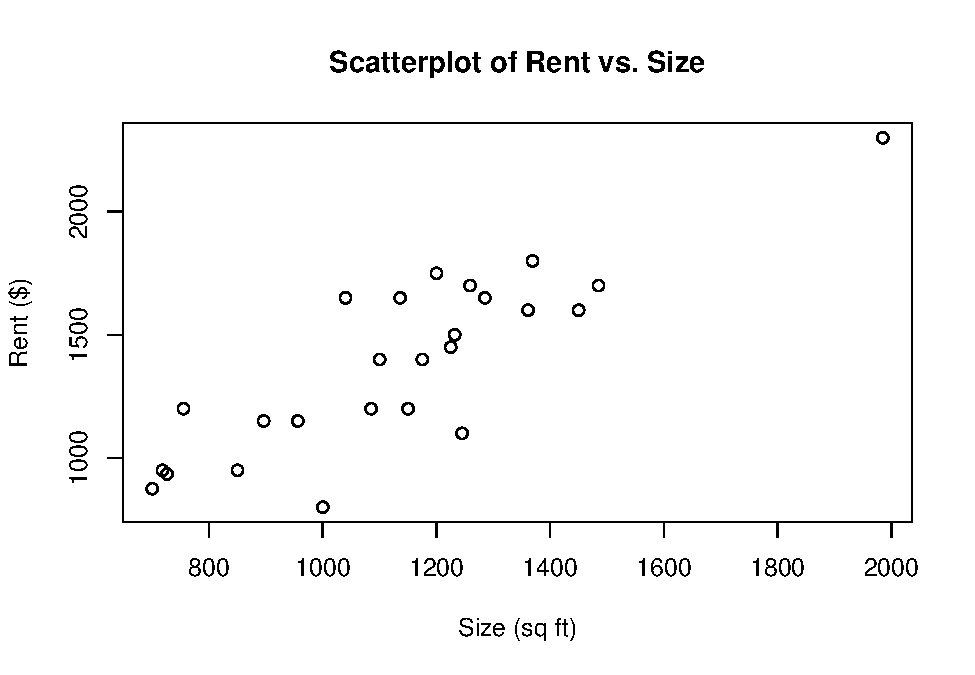
\includegraphics{Tests_and_Applications_files/figure-latex/unnamed-chunk-34-1.pdf}
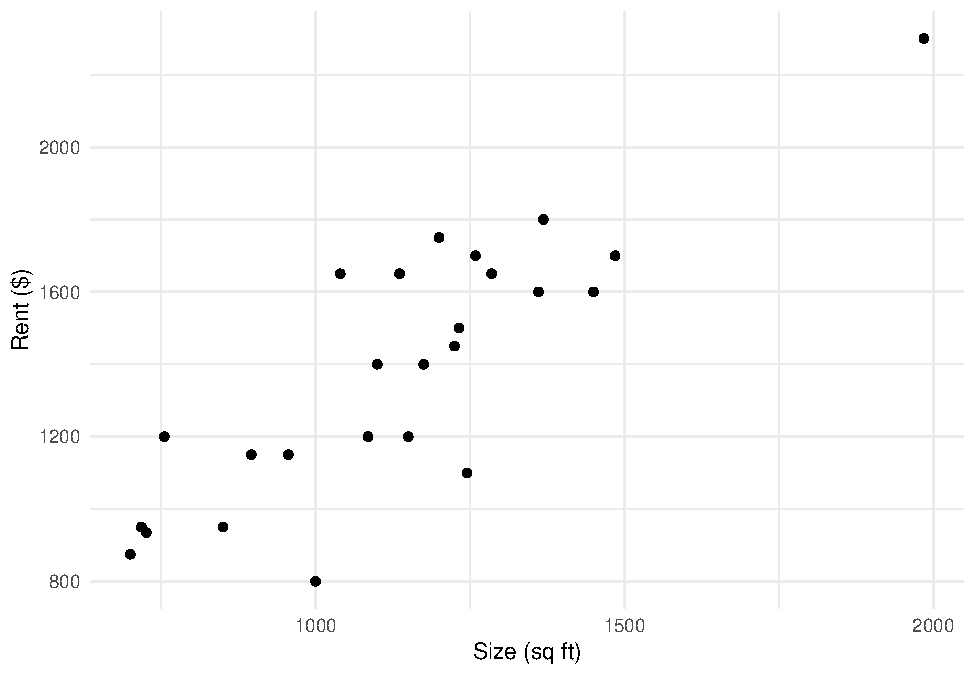
\includegraphics{Tests_and_Applications_files/figure-latex/unnamed-chunk-34-2.pdf}

The scatterplot visually inspects whether the points exhibit any pattern
or regularity.\\
\textbf{Remark}: The order of the variables in the scatter plot, i.e.,
which one is \(X\) and which one is \(Y\), is crucial in regression
analysis. This choice depends on what we want to study or verify. In the
example, the agent wants to predict rent based on size, so \texttt{size}
will be the \emph{independent variable} \(X\), and \texttt{rent} will be
the \emph{dependent variable} \(Y\).

The relationship between the two variables can be quantified using the
\emph{correlation coefficient} \(\rho\). In general, the correlation
coefficient is a measure of association between variables that ranges
from -1 to 1. Values close to -1 or 1 indicate a strong linear
relationship, while values near 0 indicate no linear relationship.

The Pearson correlation coefficient \(\rho\) can be calculated in R
using the cor function

\begin{Shaded}
\begin{Highlighting}[]
\FunctionTok{cor}\NormalTok{(data}\SpecialCharTok{$}\NormalTok{size, data}\SpecialCharTok{$}\NormalTok{rent)}
\end{Highlighting}
\end{Shaded}

\begin{verbatim}
## [1] 0.8500608
\end{verbatim}

Other types of correlation, such as Spearman or Kendall, can also be
computed:

\begin{Shaded}
\begin{Highlighting}[]
\FunctionTok{cor}\NormalTok{(data}\SpecialCharTok{$}\NormalTok{size, data}\SpecialCharTok{$}\NormalTok{rent, }\AttributeTok{method =} \StringTok{"spearman"}\NormalTok{)}
\end{Highlighting}
\end{Shaded}

\begin{verbatim}
## [1] 0.7865843
\end{verbatim}

\begin{Shaded}
\begin{Highlighting}[]
\FunctionTok{cor}\NormalTok{(data}\SpecialCharTok{$}\NormalTok{size, data}\SpecialCharTok{$}\NormalTok{rent, }\AttributeTok{method =} \StringTok{"kendall"}\NormalTok{)}
\end{Highlighting}
\end{Shaded}

\begin{verbatim}
## [1] 0.6282929
\end{verbatim}

We can set the hypothesis test with \(H_0: \rho = 0\) vs
\(H_1: \rho \not= 0\) to verify that the correlation is significant. We
can use the \texttt{cor.test} function

\begin{Shaded}
\begin{Highlighting}[]
\FunctionTok{cor.test}\NormalTok{(data}\SpecialCharTok{$}\NormalTok{size, data}\SpecialCharTok{$}\NormalTok{rent)}
\end{Highlighting}
\end{Shaded}

\begin{verbatim}
## 
##  Pearson's product-moment correlation
## 
## data:  data$size and data$rent
## t = 7.7404, df = 23, p-value = 7.518e-08
## alternative hypothesis: true correlation is not equal to 0
## 95 percent confidence interval:
##  0.6850170 0.9321097
## sample estimates:
##       cor 
## 0.8500608
\end{verbatim}

If the correlation is significantly different from zero, we can consider
the possibility of a linear relationship between the variables.

\textbf{Remark}: some of the methods for estimating and testing the
correlation coefficient are based on the assumptions that the measures
follow a \emph{bivariate normal distribution}, the distributions of
\(X\) and \(Y\) separately are normal, and the points in the scatter
plot show an elliptical shape.

\hypertarget{simple-linear-regression}{%
\subsubsection{Simple Linear
Regression}\label{simple-linear-regression}}

The Linear Regression model is commonly used to predict the value of a
numeric variable with respect to the value of another variable and it is
given as\\
\[ Y = a + b X,\] where \(a\) is called \emph{intercept} and \(b\) is
the \emph{slope}. Note that the intercept correspond to the value of
\(Y\) when \(X=0\) and the slope indicates the relative variation of
\(Y\) for each unit of \(X\). In R, the \texttt{lm} function is used to
fit a linear regression model using the \emph{least squares method}. The
syntax is \texttt{y\ \textasciitilde{}\ x}, where \(y\) is the dependent
variable and \(x\) is the independent variable.

\begin{Shaded}
\begin{Highlighting}[]
\NormalTok{model }\OtherTok{\textless{}{-}} \FunctionTok{lm}\NormalTok{(rent }\SpecialCharTok{\textasciitilde{}}\NormalTok{ size, }\AttributeTok{data =}\NormalTok{ data)}
\FunctionTok{summary}\NormalTok{(model)}
\end{Highlighting}
\end{Shaded}

\begin{verbatim}
## 
## Call:
## lm(formula = rent ~ size, data = data)
## 
## Residuals:
##     Min      1Q  Median      3Q     Max 
## -442.26  -58.86  -15.42  104.17  365.13 
## 
## Coefficients:
##             Estimate Std. Error t value Pr(>|t|)    
## (Intercept) 177.1208   161.0043    1.10    0.283    
## size          1.0651     0.1376    7.74 7.52e-08 ***
## ---
## Signif. codes:  0 '***' 0.001 '**' 0.01 '*' 0.05 '.' 0.1 ' ' 1
## 
## Residual standard error: 194.6 on 23 degrees of freedom
## Multiple R-squared:  0.7226, Adjusted R-squared:  0.7105 
## F-statistic: 59.91 on 1 and 23 DF,  p-value: 7.518e-08
\end{verbatim}

The output provides the estimated intercept and slope of the regression
line. Additionally, it performs a t.test on the slope parameter with
\(H_0: b=0\) and \(H_1:b \not= 0\).\\
The summary also report the \(R^2\) coefficient which measure the
proportion of variation in \(Y\) which is explained by \(X\). If it is
close to 1, then \(X\) predict the majority of the variability of
\(Y\).\\
We can visualize the regression line on the scatter plot:

\begin{Shaded}
\begin{Highlighting}[]
\FunctionTok{plot}\NormalTok{(data}\SpecialCharTok{$}\NormalTok{size, data}\SpecialCharTok{$}\NormalTok{rent, }\AttributeTok{main =} \StringTok{"Scatterplot with Regression Line"}\NormalTok{,}
     \AttributeTok{xlab =} \StringTok{"Size (sq ft)"}\NormalTok{, }\AttributeTok{ylab =} \StringTok{"Rent ($)"}\NormalTok{)}
\FunctionTok{abline}\NormalTok{(model, }\AttributeTok{col =} \StringTok{"red"}\NormalTok{)}
\end{Highlighting}
\end{Shaded}

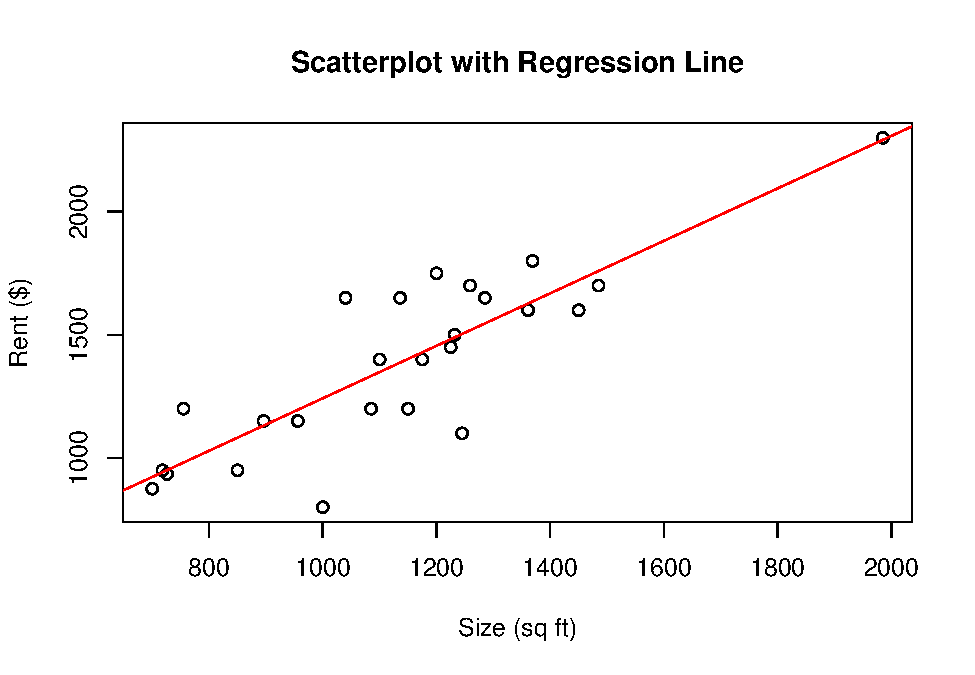
\includegraphics{Tests_and_Applications_files/figure-latex/unnamed-chunk-39-1.pdf}

\begin{Shaded}
\begin{Highlighting}[]
\FunctionTok{ggplot}\NormalTok{(data, }\FunctionTok{aes}\NormalTok{(}\AttributeTok{x=}\NormalTok{size, }\AttributeTok{y=}\NormalTok{rent))}\SpecialCharTok{+}
  \FunctionTok{geom\_point}\NormalTok{() }\SpecialCharTok{+}
  \FunctionTok{theme\_minimal}\NormalTok{() }\SpecialCharTok{+} 
  \FunctionTok{geom\_abline}\NormalTok{(}\AttributeTok{intercept =}\NormalTok{ model}\SpecialCharTok{$}\NormalTok{coefficients[}\DecValTok{1}\NormalTok{], }
              \AttributeTok{slope =}\NormalTok{ model}\SpecialCharTok{$}\NormalTok{coefficients[}\DecValTok{2}\NormalTok{], }\AttributeTok{color=}\StringTok{"red"}\NormalTok{, }
              \AttributeTok{linetype=}\StringTok{"dashed"}\NormalTok{)}
\end{Highlighting}
\end{Shaded}

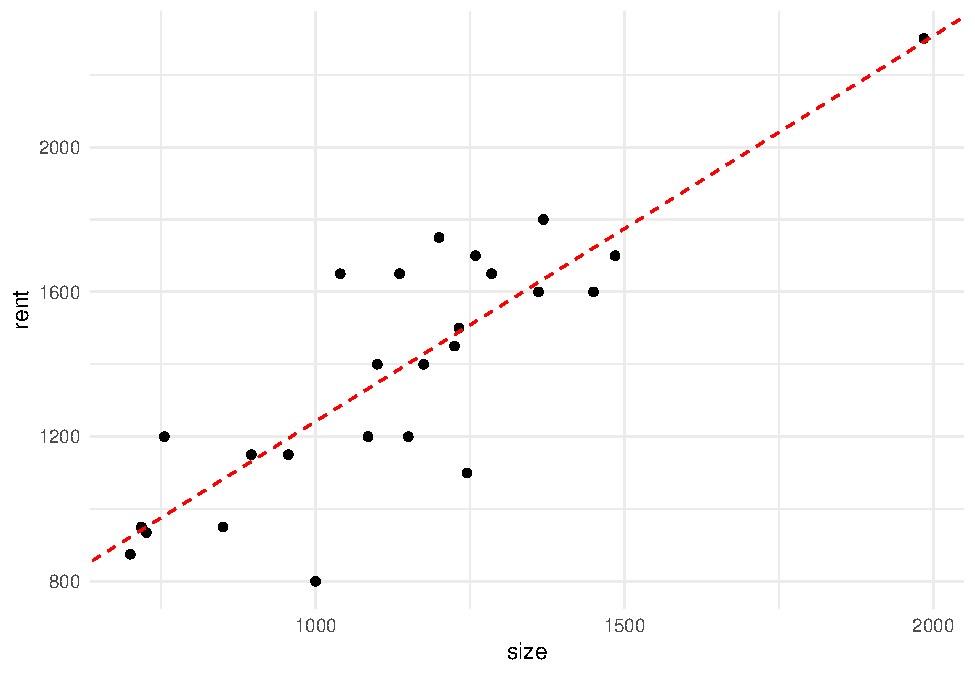
\includegraphics{Tests_and_Applications_files/figure-latex/unnamed-chunk-40-1.pdf}

Once we have the regression line, we can use the computed estimates to
predict the values of \(Y\) for specific \(X\). The \texttt{predict}
function can be used to make predictions

\begin{Shaded}
\begin{Highlighting}[]
\FunctionTok{predict}\NormalTok{(model, }\AttributeTok{newdata =} \FunctionTok{data.frame}\NormalTok{(}\AttributeTok{size =} \DecValTok{1800}\NormalTok{))}
\end{Highlighting}
\end{Shaded}

\begin{verbatim}
##       1 
## 2094.38
\end{verbatim}

Residuals measure the dispersion of points around the regression line
and are crucial to evaluate the quality of the regression model.
Considering the predicted value \(\hat{Y}_i = \hat{a} + \hat{b} X_i\)
for observation \(X_i\), the \(i\)-th residual \(e_i\) is computed as
\(e_i = Y_i- \hat{Y}_i\).\\
When using linear regression model, the following assumptions are
considered

\begin{itemize}
\tightlist
\item
  \(X\) and \(Y\) have a linear relationship.
\item
  The distribution of the possible values of \(Y\) is normal.
\item
  The variance of the values of \(Y\) is the same for each \(X\).
\end{itemize}

These can be verified analyzing the residuals.

\begin{Shaded}
\begin{Highlighting}[]
\FunctionTok{plot}\NormalTok{(model}\SpecialCharTok{$}\NormalTok{fitted.values, model}\SpecialCharTok{$}\NormalTok{residuals, }\AttributeTok{main =} \StringTok{"Residuals vs Fitted"}\NormalTok{,}
     \AttributeTok{xlab =} \StringTok{"Fitted Values"}\NormalTok{, }\AttributeTok{ylab =} \StringTok{"Residuals"}\NormalTok{)}
\FunctionTok{abline}\NormalTok{(}\AttributeTok{h =} \DecValTok{0}\NormalTok{, }\AttributeTok{col =} \StringTok{"red"}\NormalTok{)}
\end{Highlighting}
\end{Shaded}

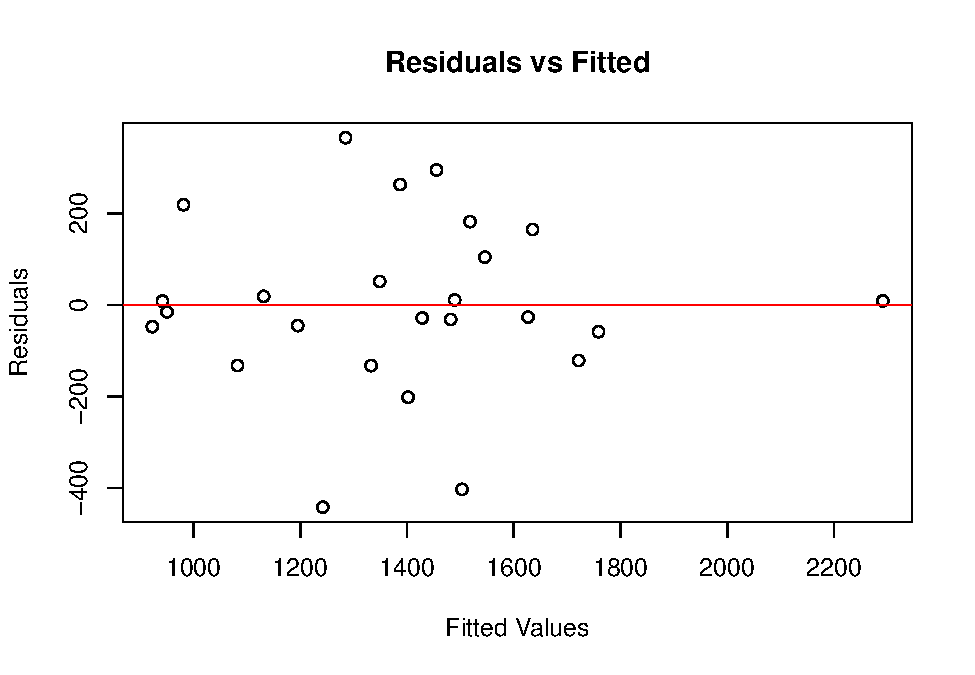
\includegraphics{Tests_and_Applications_files/figure-latex/unnamed-chunk-42-1.pdf}

Alternatively, we can also investigate the quantiles of the residuals
using a qqplot.

\begin{Shaded}
\begin{Highlighting}[]
\FunctionTok{qqnorm}\NormalTok{(model}\SpecialCharTok{$}\NormalTok{residuals)}
\FunctionTok{qqline}\NormalTok{(model}\SpecialCharTok{$}\NormalTok{residuals, }\AttributeTok{col =} \StringTok{"red"}\NormalTok{)}
\end{Highlighting}
\end{Shaded}

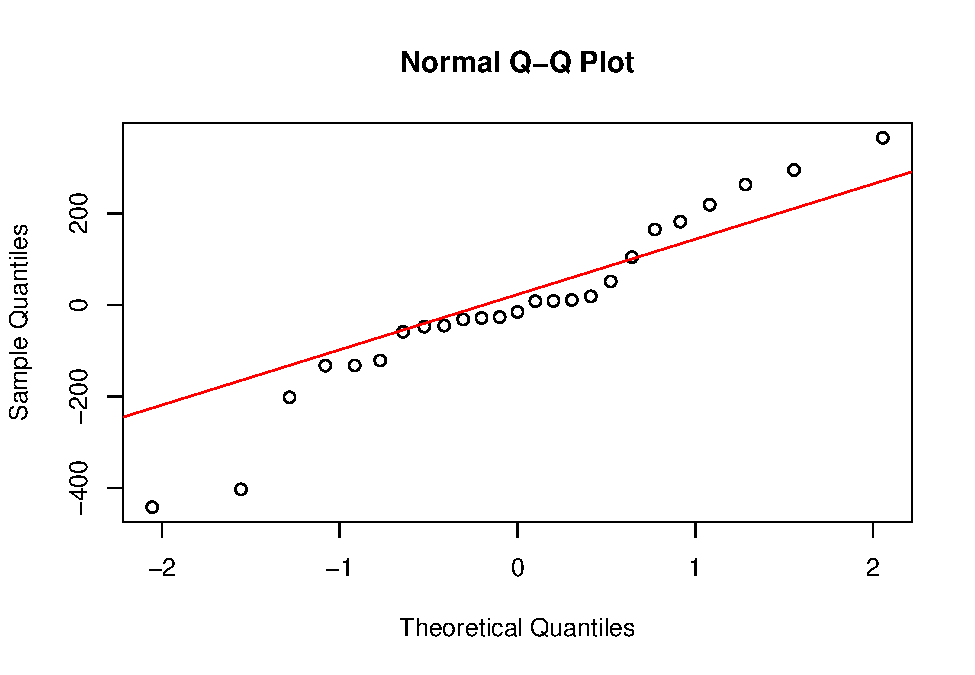
\includegraphics{Tests_and_Applications_files/figure-latex/unnamed-chunk-43-1.pdf}

If the normality assumptions are satisfied, residuals should concentrate
around the line \(Y=0\) and an equivalent dispersion of points above and
below the line.

\hypertarget{confidence-and-prediction-bands}{%
\paragraph{Confidence and Prediction
Bands}\label{confidence-and-prediction-bands}}

To assess uncertainty in the regression estimates, we calculate
confidence and prediction intervals using the predict function with the
interval argument

\begin{Shaded}
\begin{Highlighting}[]
\NormalTok{newdat }\OtherTok{\textless{}{-}} \FunctionTok{data.frame}\NormalTok{(}\AttributeTok{size=}\FunctionTok{seq}\NormalTok{(}\DecValTok{250}\NormalTok{, }\DecValTok{2200}\NormalTok{, }\DecValTok{10}\NormalTok{))}
\CommentTok{\# Confidence intervals}
\NormalTok{conf\_int }\OtherTok{\textless{}{-}} \FunctionTok{predict}\NormalTok{(model, }\AttributeTok{interval =} \StringTok{"confidence"}\NormalTok{, }\AttributeTok{newdata =}\NormalTok{ newdat)}

\CommentTok{\# Prediction intervals}
\NormalTok{pred\_int }\OtherTok{\textless{}{-}} \FunctionTok{predict}\NormalTok{(model, }\AttributeTok{interval =} \StringTok{"prediction"}\NormalTok{, }\AttributeTok{newdata =}\NormalTok{ newdat)}

\CommentTok{\# Visualizing intervals}
\FunctionTok{plot}\NormalTok{(data}\SpecialCharTok{$}\NormalTok{size, data}\SpecialCharTok{$}\NormalTok{rent, }\AttributeTok{main =} \StringTok{"Confidence and Prediction Intervals"}\NormalTok{,}
     \AttributeTok{xlab =} \StringTok{"Size (sq ft)"}\NormalTok{, }\AttributeTok{ylab =} \StringTok{"Rent ($)"}\NormalTok{)}
\FunctionTok{abline}\NormalTok{(model, }\AttributeTok{lty =} \DecValTok{2}\NormalTok{)}
\FunctionTok{lines}\NormalTok{(newdat}\SpecialCharTok{$}\NormalTok{size, conf\_int[, }\DecValTok{2}\NormalTok{], }\AttributeTok{col =} \StringTok{"blue"}\NormalTok{, }\AttributeTok{lty =} \DecValTok{2}\NormalTok{)}
\FunctionTok{lines}\NormalTok{(newdat}\SpecialCharTok{$}\NormalTok{size, conf\_int[, }\DecValTok{3}\NormalTok{], }\AttributeTok{col =} \StringTok{"blue"}\NormalTok{, }\AttributeTok{lty =} \DecValTok{2}\NormalTok{)}
\FunctionTok{lines}\NormalTok{(newdat}\SpecialCharTok{$}\NormalTok{size, pred\_int[, }\DecValTok{2}\NormalTok{], }\AttributeTok{col =} \StringTok{"red"}\NormalTok{, }\AttributeTok{lty =} \DecValTok{3}\NormalTok{)}
\FunctionTok{lines}\NormalTok{(newdat}\SpecialCharTok{$}\NormalTok{size, pred\_int[, }\DecValTok{3}\NormalTok{], }\AttributeTok{col =} \StringTok{"red"}\NormalTok{, }\AttributeTok{lty =} \DecValTok{3}\NormalTok{)}
\end{Highlighting}
\end{Shaded}

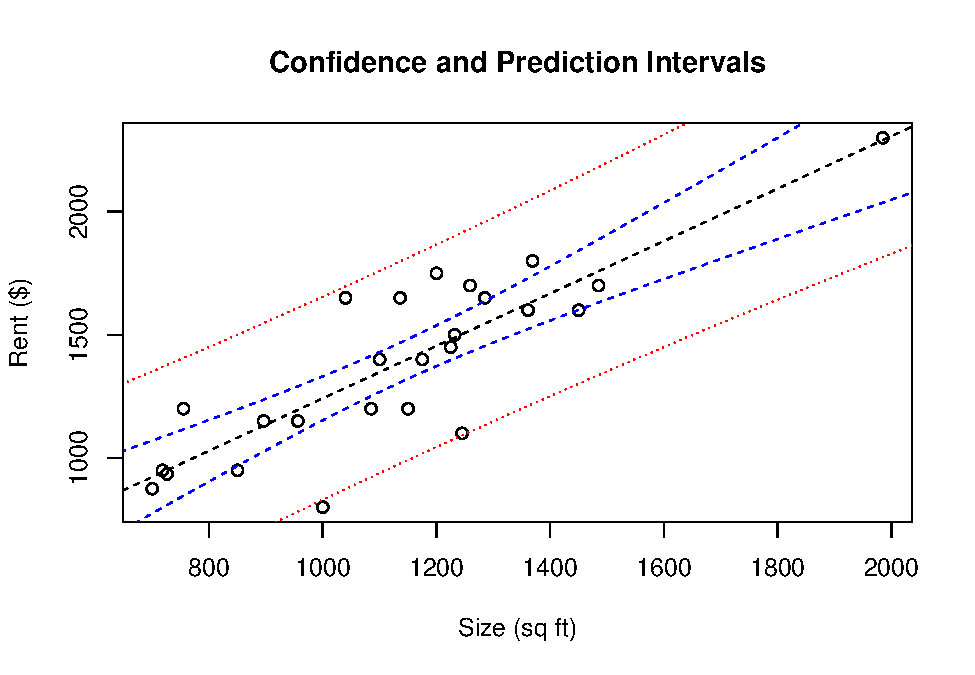
\includegraphics{Tests_and_Applications_files/figure-latex/unnamed-chunk-44-1.pdf}

\hypertarget{correlation-and-cause-effect}{%
\subsubsection{Correlation and
Cause-Effect}\label{correlation-and-cause-effect}}

If two events are associated, one wonders if there is the possibility
that one is the cause for the other. Notice that the presence of
correlation between two variables does not imply a cause-effect
relation, but for example it can be due to some common cause.

One possibility is the presence of \emph{confounding variables}, that is
a non-measured variable which is related to one or more of the measured
variables.

\hypertarget{robust-statistics-1}{%
\subsubsection{Robust Statistics}\label{robust-statistics-1}}

The classical linear regression method, Ordinary Least Squares (OLS), is
highly sensitive to violations of the assumptions. For example in
presence of outliers, non-normality of errors, heteroscedasticity, that
is constant variance of errors. Robust linear regression methods address
these challenges by reducing the influence of outliers and when
assumptions are violated. Furthermore, robust methods are designed such
that they perform equivalently ot the OLS method if all the assumptions
are satisfied.\\
Common approaches include

\begin{itemize}
\tightlist
\item
  \emph{M-Estimators}: Generalization of maximum likelihood estimators,
  minimizing a robust loss function.
\end{itemize}

\begin{Shaded}
\begin{Highlighting}[]
\FunctionTok{library}\NormalTok{(MASS)}
\NormalTok{modelM }\OtherTok{\textless{}{-}} \FunctionTok{rlm}\NormalTok{(rent }\SpecialCharTok{\textasciitilde{}}\NormalTok{ size, }\AttributeTok{data =}\NormalTok{ data)}
\FunctionTok{summary}\NormalTok{(modelM)}
\end{Highlighting}
\end{Shaded}

\begin{verbatim}
## 
## Call: rlm(formula = rent ~ size, data = data)
## Residuals:
##     Min      1Q  Median      3Q     Max 
## -447.43  -65.52  -19.74   98.12  359.84 
## 
## Coefficients:
##             Value    Std. Error t value 
## (Intercept) 179.2019 157.2227     1.1398
## size          1.0682   0.1344     7.9495
## 
## Residual standard error: 145.5 on 23 degrees of freedom
\end{verbatim}

\begin{itemize}
\tightlist
\item
  \emph{MM-Estimators}: Improves robustness by combining high breakdown
  point and high efficiency.
\end{itemize}

\begin{Shaded}
\begin{Highlighting}[]
\FunctionTok{library}\NormalTok{(robustbase)}
\NormalTok{modelMM }\OtherTok{\textless{}{-}} \FunctionTok{lmrob}\NormalTok{(rent }\SpecialCharTok{\textasciitilde{}}\NormalTok{ size, }\AttributeTok{data =}\NormalTok{ data)}
\FunctionTok{summary}\NormalTok{(modelMM)}
\end{Highlighting}
\end{Shaded}

\begin{verbatim}
## 
## Call:
## lmrob(formula = rent ~ size, data = data)
##  \--> method = "MM"
## Residuals:
##     Min      1Q  Median      3Q     Max 
## -450.20  -67.30  -23.07   95.94  357.15 
## 
## Coefficients:
##              Estimate Std. Error t value Pr(>|t|)    
## (Intercept) 184.02581   82.29594   2.236   0.0353 *  
## size          1.06618    0.06146  17.347 1.05e-14 ***
## ---
## Signif. codes:  0 '***' 0.001 '**' 0.01 '*' 0.05 '.' 0.1 ' ' 1
## 
## Robust residual standard error: 155.4 
## Multiple R-squared:  0.7708, Adjusted R-squared:  0.7608 
## Convergence in 12 IRWLS iterations
## 
## Robustness weights: 
##  4 weights are ~= 1. The remaining 21 ones are summarized as
##    Min. 1st Qu.  Median    Mean 3rd Qu.    Max. 
##  0.3815  0.8391  0.9271  0.8608  0.9893  0.9980 
## Algorithmic parameters: 
##        tuning.chi                bb        tuning.psi        refine.tol 
##         1.548e+00         5.000e-01         4.685e+00         1.000e-07 
##           rel.tol         scale.tol         solve.tol          zero.tol 
##         1.000e-07         1.000e-10         1.000e-07         1.000e-10 
##       eps.outlier             eps.x warn.limit.reject warn.limit.meanrw 
##         4.000e-03         3.611e-09         5.000e-01         5.000e-01 
##      nResample         max.it       best.r.s       k.fast.s          k.max 
##            500             50              2              1            200 
##    maxit.scale      trace.lev            mts     compute.rd fast.s.large.n 
##            200              0           1000              0           2000 
##                   psi           subsampling                   cov 
##            "bisquare"         "nonsingular"         ".vcov.avar1" 
## compute.outlier.stats 
##                  "SM" 
## seed : int(0)
\end{verbatim}

\begin{itemize}
\tightlist
\item
  \emph{Least Trimmed Squares (LTS)}: Minimizes the sum of the smallest
  squared residuals, focusing on a subset of data.
\end{itemize}

\begin{Shaded}
\begin{Highlighting}[]
\FunctionTok{library}\NormalTok{(robustbase)}
\NormalTok{model }\OtherTok{\textless{}{-}} \FunctionTok{ltsReg}\NormalTok{(rent }\SpecialCharTok{\textasciitilde{}}\NormalTok{ size, }\AttributeTok{data =}\NormalTok{ data)}
\FunctionTok{summary}\NormalTok{(model)}
\end{Highlighting}
\end{Shaded}

\begin{verbatim}
## 
## Call:
## ltsReg.formula(formula = rent ~ size, data = data)
## 
## Residuals (from reweighted LS):
##     Min      1Q  Median      3Q     Max 
## -223.95  -65.67  -11.98   81.12  344.15 
## 
## Coefficients:
##           Estimate Std. Error t value Pr(>|t|)    
## Intercept 189.3257   127.3755   1.486    0.152    
## size        1.0736     0.1085   9.891 2.35e-09 ***
## ---
## Signif. codes:  0 '***' 0.001 '**' 0.01 '*' 0.05 '.' 0.1 ' ' 1
## 
## Residual standard error: 152.3 on 21 degrees of freedom
## Multiple R-Squared: 0.8233,  Adjusted R-squared: 0.8149 
## F-statistic: 97.83 on 1 and 21 DF,  p-value: 2.347e-09
\end{verbatim}

\begin{itemize}
\tightlist
\item
  \emph{Quantile Regression}: Models conditional quantiles (e.g., median
  or other percentiles) rather than the mean.
\end{itemize}

\begin{Shaded}
\begin{Highlighting}[]
\FunctionTok{library}\NormalTok{(quantreg)}
\NormalTok{model }\OtherTok{\textless{}{-}} \FunctionTok{rq}\NormalTok{(rent }\SpecialCharTok{\textasciitilde{}}\NormalTok{ size, }\AttributeTok{data =}\NormalTok{ data, }\AttributeTok{tau =} \FloatTok{0.5}\NormalTok{)  }\CommentTok{\# Median regression}
\FunctionTok{summary}\NormalTok{(model)}
\end{Highlighting}
\end{Shaded}

\begin{verbatim}
## 
## Call: rq(formula = rent ~ size, tau = 0.5, data = data)
## 
## tau: [1] 0.5
## 
## Coefficients:
##             coefficients lower bd  upper bd 
## (Intercept) 147.87530     96.42451 291.64525
## size          1.08419      0.95750   1.13032
\end{verbatim}

\begin{itemize}
\tightlist
\item
  \emph{Bayesian Robust Regression}: Bayesian approach to robust
  regression using heavy-tailed distributions (e.g., t-distribution).
\end{itemize}

\begin{Shaded}
\begin{Highlighting}[]
\FunctionTok{library}\NormalTok{(brms)}
\NormalTok{model }\OtherTok{\textless{}{-}} \FunctionTok{brm}\NormalTok{(rent }\SpecialCharTok{\textasciitilde{}}\NormalTok{ size, }\AttributeTok{data =}\NormalTok{ data, }\AttributeTok{family =} \FunctionTok{student}\NormalTok{())}
\end{Highlighting}
\end{Shaded}

\begin{verbatim}
## 
## SAMPLING FOR MODEL 'anon_model' NOW (CHAIN 1).
## Chain 1: 
## Chain 1: Gradient evaluation took 3.8e-05 seconds
## Chain 1: 1000 transitions using 10 leapfrog steps per transition would take 0.38 seconds.
## Chain 1: Adjust your expectations accordingly!
## Chain 1: 
## Chain 1: 
## Chain 1: Iteration:    1 / 2000 [  0%]  (Warmup)
## Chain 1: Iteration:  200 / 2000 [ 10%]  (Warmup)
## Chain 1: Iteration:  400 / 2000 [ 20%]  (Warmup)
## Chain 1: Iteration:  600 / 2000 [ 30%]  (Warmup)
## Chain 1: Iteration:  800 / 2000 [ 40%]  (Warmup)
## Chain 1: Iteration: 1000 / 2000 [ 50%]  (Warmup)
## Chain 1: Iteration: 1001 / 2000 [ 50%]  (Sampling)
## Chain 1: Iteration: 1200 / 2000 [ 60%]  (Sampling)
## Chain 1: Iteration: 1400 / 2000 [ 70%]  (Sampling)
## Chain 1: Iteration: 1600 / 2000 [ 80%]  (Sampling)
## Chain 1: Iteration: 1800 / 2000 [ 90%]  (Sampling)
## Chain 1: Iteration: 2000 / 2000 [100%]  (Sampling)
## Chain 1: 
## Chain 1:  Elapsed Time: 0.128 seconds (Warm-up)
## Chain 1:                0.04 seconds (Sampling)
## Chain 1:                0.168 seconds (Total)
## Chain 1: 
## 
## SAMPLING FOR MODEL 'anon_model' NOW (CHAIN 2).
## Chain 2: 
## Chain 2: Gradient evaluation took 7e-06 seconds
## Chain 2: 1000 transitions using 10 leapfrog steps per transition would take 0.07 seconds.
## Chain 2: Adjust your expectations accordingly!
## Chain 2: 
## Chain 2: 
## Chain 2: Iteration:    1 / 2000 [  0%]  (Warmup)
## Chain 2: Iteration:  200 / 2000 [ 10%]  (Warmup)
## Chain 2: Iteration:  400 / 2000 [ 20%]  (Warmup)
## Chain 2: Iteration:  600 / 2000 [ 30%]  (Warmup)
## Chain 2: Iteration:  800 / 2000 [ 40%]  (Warmup)
## Chain 2: Iteration: 1000 / 2000 [ 50%]  (Warmup)
## Chain 2: Iteration: 1001 / 2000 [ 50%]  (Sampling)
## Chain 2: Iteration: 1200 / 2000 [ 60%]  (Sampling)
## Chain 2: Iteration: 1400 / 2000 [ 70%]  (Sampling)
## Chain 2: Iteration: 1600 / 2000 [ 80%]  (Sampling)
## Chain 2: Iteration: 1800 / 2000 [ 90%]  (Sampling)
## Chain 2: Iteration: 2000 / 2000 [100%]  (Sampling)
## Chain 2: 
## Chain 2:  Elapsed Time: 0.123 seconds (Warm-up)
## Chain 2:                0.044 seconds (Sampling)
## Chain 2:                0.167 seconds (Total)
## Chain 2: 
## 
## SAMPLING FOR MODEL 'anon_model' NOW (CHAIN 3).
## Chain 3: 
## Chain 3: Gradient evaluation took 7e-06 seconds
## Chain 3: 1000 transitions using 10 leapfrog steps per transition would take 0.07 seconds.
## Chain 3: Adjust your expectations accordingly!
## Chain 3: 
## Chain 3: 
## Chain 3: Iteration:    1 / 2000 [  0%]  (Warmup)
## Chain 3: Iteration:  200 / 2000 [ 10%]  (Warmup)
## Chain 3: Iteration:  400 / 2000 [ 20%]  (Warmup)
## Chain 3: Iteration:  600 / 2000 [ 30%]  (Warmup)
## Chain 3: Iteration:  800 / 2000 [ 40%]  (Warmup)
## Chain 3: Iteration: 1000 / 2000 [ 50%]  (Warmup)
## Chain 3: Iteration: 1001 / 2000 [ 50%]  (Sampling)
## Chain 3: Iteration: 1200 / 2000 [ 60%]  (Sampling)
## Chain 3: Iteration: 1400 / 2000 [ 70%]  (Sampling)
## Chain 3: Iteration: 1600 / 2000 [ 80%]  (Sampling)
## Chain 3: Iteration: 1800 / 2000 [ 90%]  (Sampling)
## Chain 3: Iteration: 2000 / 2000 [100%]  (Sampling)
## Chain 3: 
## Chain 3:  Elapsed Time: 0.123 seconds (Warm-up)
## Chain 3:                0.038 seconds (Sampling)
## Chain 3:                0.161 seconds (Total)
## Chain 3: 
## 
## SAMPLING FOR MODEL 'anon_model' NOW (CHAIN 4).
## Chain 4: 
## Chain 4: Gradient evaluation took 7e-06 seconds
## Chain 4: 1000 transitions using 10 leapfrog steps per transition would take 0.07 seconds.
## Chain 4: Adjust your expectations accordingly!
## Chain 4: 
## Chain 4: 
## Chain 4: Iteration:    1 / 2000 [  0%]  (Warmup)
## Chain 4: Iteration:  200 / 2000 [ 10%]  (Warmup)
## Chain 4: Iteration:  400 / 2000 [ 20%]  (Warmup)
## Chain 4: Iteration:  600 / 2000 [ 30%]  (Warmup)
## Chain 4: Iteration:  800 / 2000 [ 40%]  (Warmup)
## Chain 4: Iteration: 1000 / 2000 [ 50%]  (Warmup)
## Chain 4: Iteration: 1001 / 2000 [ 50%]  (Sampling)
## Chain 4: Iteration: 1200 / 2000 [ 60%]  (Sampling)
## Chain 4: Iteration: 1400 / 2000 [ 70%]  (Sampling)
## Chain 4: Iteration: 1600 / 2000 [ 80%]  (Sampling)
## Chain 4: Iteration: 1800 / 2000 [ 90%]  (Sampling)
## Chain 4: Iteration: 2000 / 2000 [100%]  (Sampling)
## Chain 4: 
## Chain 4:  Elapsed Time: 0.113 seconds (Warm-up)
## Chain 4:                0.042 seconds (Sampling)
## Chain 4:                0.155 seconds (Total)
## Chain 4:
\end{verbatim}

\begin{Shaded}
\begin{Highlighting}[]
\FunctionTok{summary}\NormalTok{(model)}
\end{Highlighting}
\end{Shaded}

\begin{verbatim}
##  Family: student 
##   Links: mu = identity; sigma = identity; nu = identity 
## Formula: rent ~ size 
##    Data: data (Number of observations: 25) 
##   Draws: 4 chains, each with iter = 2000; warmup = 1000; thin = 1;
##          total post-warmup draws = 4000
## 
## Regression Coefficients:
##           Estimate Est.Error l-95% CI u-95% CI Rhat Bulk_ESS Tail_ESS
## Intercept   181.40    158.37  -144.21   500.30 1.00     4132     2587
## size          1.06      0.13     0.79     1.33 1.00     4083     2739
## 
## Further Distributional Parameters:
##       Estimate Est.Error l-95% CI u-95% CI Rhat Bulk_ESS Tail_ESS
## sigma   186.33     33.61   126.25   261.11 1.00     2272     1697
## nu       20.12     14.05     3.37    57.02 1.00     2957     2046
## 
## Draws were sampled using sampling(NUTS). For each parameter, Bulk_ESS
## and Tail_ESS are effective sample size measures, and Rhat is the potential
## scale reduction factor on split chains (at convergence, Rhat = 1).
\end{verbatim}

\begin{itemize}
\tightlist
\item
  \emph{Nonparametric Regression} (Locally Weighted): Fits locally
  weighted regression models.
\end{itemize}

\begin{Shaded}
\begin{Highlighting}[]
\FunctionTok{library}\NormalTok{(stats)}
\NormalTok{model }\OtherTok{\textless{}{-}} \FunctionTok{loess}\NormalTok{(rent }\SpecialCharTok{\textasciitilde{}}\NormalTok{ size, }\AttributeTok{data =}\NormalTok{ data)}
\FunctionTok{summary}\NormalTok{(model)}
\end{Highlighting}
\end{Shaded}

\begin{verbatim}
## Call:
## loess(formula = rent ~ size, data = data)
## 
## Number of Observations: 25 
## Equivalent Number of Parameters: 5.14 
## Residual Standard Error: 210.4 
## Trace of smoother matrix: 5.66  (exact)
## 
## Control settings:
##   span     :  0.75 
##   degree   :  2 
##   family   :  gaussian
##   surface  :  interpolate      cell = 0.2
##   normalize:  TRUE
##  parametric:  FALSE
## drop.square:  FALSE
\end{verbatim}

\hypertarget{exercises}{%
\subsection{Exercises}\label{exercises}}

\begin{enumerate}
\def\labelenumi{\arabic{enumi}.}
\tightlist
\item
  Perform a linear regression analysis using the following data
\end{enumerate}

\begin{Shaded}
\begin{Highlighting}[]
\NormalTok{height }\OtherTok{\textless{}{-}} \FunctionTok{c}\NormalTok{(}\DecValTok{175}\NormalTok{, }\DecValTok{168}\NormalTok{, }\DecValTok{170}\NormalTok{, }\DecValTok{171}\NormalTok{, }\DecValTok{169}\NormalTok{, }\DecValTok{165}\NormalTok{, }\DecValTok{165}\NormalTok{, }\DecValTok{160}\NormalTok{, }\DecValTok{180}\NormalTok{, }\DecValTok{186}\NormalTok{)}
\NormalTok{weight }\OtherTok{\textless{}{-}} \FunctionTok{c}\NormalTok{(}\DecValTok{80}\NormalTok{, }\DecValTok{68}\NormalTok{, }\DecValTok{72}\NormalTok{, }\DecValTok{75}\NormalTok{, }\DecValTok{70}\NormalTok{, }\DecValTok{65}\NormalTok{, }\DecValTok{62}\NormalTok{, }\DecValTok{60}\NormalTok{, }\DecValTok{85}\NormalTok{, }\DecValTok{90}\NormalTok{)}
\end{Highlighting}
\end{Shaded}

\begin{enumerate}
\def\labelenumi{\arabic{enumi}.}
\setcounter{enumi}{1}
\tightlist
\item
  Regression of Carbon Content and Yield Strength. Conduct a linear
  regression analysis for the following data
\end{enumerate}

\begin{Shaded}
\begin{Highlighting}[]
\NormalTok{carbon }\OtherTok{\textless{}{-}} \FunctionTok{c}\NormalTok{(}\DecValTok{46}\NormalTok{, }\DecValTok{27}\NormalTok{, }\DecValTok{44}\NormalTok{, }\DecValTok{35}\NormalTok{, }\DecValTok{35}\NormalTok{, }\DecValTok{25}\NormalTok{, }\DecValTok{34}\NormalTok{, }\DecValTok{29}\NormalTok{, }\DecValTok{34}\NormalTok{)}
\NormalTok{yield }\OtherTok{\textless{}{-}} \FunctionTok{c}\NormalTok{(}\DecValTok{71}\NormalTok{, }\DecValTok{47}\NormalTok{, }\DecValTok{63}\NormalTok{, }\DecValTok{52}\NormalTok{, }\DecValTok{55}\NormalTok{, }\DecValTok{37}\NormalTok{, }\DecValTok{49}\NormalTok{, }\DecValTok{43}\NormalTok{, }\DecValTok{48}\NormalTok{)}
\end{Highlighting}
\end{Shaded}

\hypertarget{references}{%
\subsection*{References}\label{references}}
\addcontentsline{toc}{subsection}{References}

\hypertarget{refs}{}
\begin{CSLReferences}{1}{0}
\leavevmode\vadjust pre{\hypertarget{ref-wasserstein2019moving}{}}%
Wasserstein, RL. 2019. {``Moving to a World Beyond {`p\textless{}
0.05'}.''} Taylor \& Francis.

\leavevmode\vadjust pre{\hypertarget{ref-wilcox2018guide}{}}%
Wilcox, Rand R, and Guillaume A Rousselet. 2018. {``A Guide to Robust
Statistical Methods in Neuroscience.''} \emph{Current Protocols in
Neuroscience} 82 (1): 8--42.

\leavevmode\vadjust pre{\hypertarget{ref-yu2022beyond}{}}%
Yu, Zhaoxia, Michele Guindani, Steven F Grieco, Lujia Chen, Todd C
Holmes, and Xiangmin Xu. 2022. {``Beyond t Test and ANOVA: Applications
of Mixed-Effects Models for More Rigorous Statistical Analysis in
Neuroscience Research.''} \emph{Neuron} 110 (1): 21--35.

\end{CSLReferences}

\end{document}
